%MIT License
%
%Copyright (c) 2018 Chen Wang [https://chenwang.site]
%
%Permission is hereby granted, free of charge, to any person obtaining a copy
%of this software and associated documentation files (the "Software"), to deal
%in the Software without restriction, including without limitation the rights
%to use, copy, modify, merge, publish, distribute, sublicense, and/or sell
%copies of the Software, and to permit persons to whom the Software is
%furnished to do so, subject to the following conditions:
%
%The above copyright notice and this permission notice shall be included in all
%copies or substantial portions of the Software.
%
%THE SOFTWARE IS PROVIDED "AS IS", WITHOUT WARRANTY OF ANY KIND, EXPRESS OR
%IMPLIED, INCLUDING BUT NOT LIMITED TO THE WARRANTIES OF MERCHANTABILITY,
%FITNESS FOR A PARTICULAR PURPOSE AND NONINFRINGEMENT. IN NO EVENT SHALL THE
%AUTHORS OR COPYRIGHT HOLDERS BE LIABLE FOR ANY CLAIM, DAMAGES OR OTHER
%LIABILITY, WHETHER IN AN ACTION OF CONTRACT, TORT OR OTHERWISE, ARISING FROM,
%OUT OF OR IN CONNECTION WITH THE SOFTWARE OR THE USE OR OTHER DEALINGS IN THE
%SOFTWARE.
\documentclass[12pt,a4paper,oneside]{Thesis} % Paper size, default font size and one-sided paper

\graphicspath{%
	{./Pictures/}%
	{./Figures/}%
}
\DeclareMathOperator{\Tr}{Tr}
\let\savedegree\degree
\let\degree\relax
\let\savedegree\ref
\let\rem\relax
\usepackage{adjustbox}
\usepackage{amsmath}
\usepackage[amssymb]{SIunits}
\usepackage{amssymb}
\usepackage{multirow}
\usepackage{wrapfig}
\usepackage{enumitem}
\usepackage{subcaption}
\usepackage{mathtools}
\usepackage{lipsum}
\usepackage{hyperref}
\usepackage[ruled,vlined,noresetcount]{algorithm2e}
%\usepackage{algpseudocode}
\usepackage[square, numbers, comma, sort&compress]{natbib} % Use the natbib reference package - read up on this to edit the reference style; if you want text (e.g. Smith et al., 2012) for the in-text references (instead of numbers), remove 'numbers'

\title{\ttitle} % Defines the thesis title - don't touch this

%extra packages
\usepackage{float}
\usepackage{color,soul}               % highlighting text
\usepackage{enumerate}
\usepackage{Styles/mydefs}


\begin{document}

\frontmatter % Use roman page numbering style (i, ii, iii, iv...) for the pre-content pages

\setstretch{1.3} % Line spacing of 1.3
% Define the page headers using the Fr package and set up for one-sided printing

\pagestyle{fancy} % Finally, use the "fancy" page style to implement the FancyHdr headers
\fancyhead{}   %clear all fields
\fancyhead[LO]{\sl{\leftmark}}
\fancyhead[RE]{\sl{\rightmark}}
\fancyhead[LE,RO]{\thepage}


%----------------------------------------------------------------------------------------
%	TITLE PAGE
%----------------------------------------------------------------------------------------

%%% Use \maketitleforreview instead of \maketitle, if you want a PLAIN TITLE PAGE

\maketitle
% \maketitleforreview


% ----------------------------------------------------------------------------------------
% 	DECLARATION PAGE
% ----------------------------------------------------------------------------------------

%\thesisdeclareOriginality{I hereby certify that the work embodied in this thesis is the result of original research, is free of plagiarised materials, and has not been submitted for a higher degree to any other University or Institution.}{Aug. 2018}{Styles/signature.png}
%
%\thesisdeclareSupervisor{I have reviewed the content and presentation style of this thesis and declare it is free of plagiarism and of sufficient grammatical clarity to be examined.  To the best of my knowledge, the research and writing are those of the candidate except as acknowledged in the Author Attribution Statement. I confirm that the investigations were conducted in accord with the ethics policies and integrity standards of Nanyang Technological University and that the research data are presented honestly and without prejudice.}{Mar. 2019}{Styles/signature.png}
%
%\thesisdeclareAuthorship{Please select one of the following; *delete as appropriate:
%\\
%*(A) This thesis does not contain any materials from papers published in peer-reviewed journals or from papers accepted at conferences in which I am listed as an author.
%\\
%*(B) This thesis contains material from [x number] paper(s) published in the following peer-reviewed journal(s) / from papers accepted at conferences in which I am listed as an author.}
%{Please amend the typical statements below to suit your circumstances if (B) is selected.
%
%	Chapter 4 is published as {\color{blue}D.T. Murphy, S. Schmid, J.R. Hester, P.E.R. Blanchard, and W. Miiller.  Coordination site disorder in spinel-type LiMnTiO4.  Inorganic Chemistry 54, 4636-4643 (2015). DOI: 10.1021/ic502747p.}
%
%	The contributions of the co-authors are as follows:
%	\begin{itemize}[topsep=1pt,itemsep=1pt,partopsep=1pt, parsep=1pt]
%		\item A/Prof Schmid provided the initial project direction and edited the manuscript drafts.
%		\item I prepared the manuscript drafts.  The manuscript was revised by Dr Hester and Dr. Blanchard.
%		\item I co-designed the study with A/Prof Siegbert Schmid and performed all the laboratory work at the School of Materials Science and Engineering and the Singapore Synchrotron Light Source.   I also analyzed the data.
%		\item All microscopy, including sample preparation, was conducted by me in the Facility for Analysis, Characterization, Testing and Simulation.
%		\item Dr James Hester assisted in the collection of the neutron powder diffraction data.
%		\item Dr Peter Blanchard assisted in the interpretation of the X-ray absorption spectroscopy data and carried out the spectral interpretation.
%		\item Dr Wojciech Miiller assisted in the collection and provide guidance in the interpretation of the magnetic measurement data.
%	\end{itemize}
%
%	Chapter 5 is published as {\color{blue}H. V Doan, B. Yao, Y. Fang, A. Sartbaeva, U. Hintermair, V. P Ting, Controlled Formation of Hierarchical Metal-Organic Frameworks using CO2 Expanded Solvent Systems. In press, ACS Sustainable Chemistry \& Engineering (2017). DOI: 10.1021/acssuschemeng.7b01429}
%
%	The contributions of the co-authors are as follows:
%	\begin{itemize}[topsep=1pt,itemsep=1pt,partopsep=1pt, parsep=1pt]
%		\item Prof Ting suggested the materials area and edited the manuscript drafts.
%		\item I wrote the drafts of the manuscript.  The manuscript was revised together with Dr. Sartbaeva and Dr. Yao.
%		\item II performed all the materials synthesis, collected X-ray diffraction patterns and visible light spectra, carried transmission electron microscopy, and conducted data evaluation.
%		\item IDr. Y. Fang conducted the Rietveld analysis of the powder X-ray diffraction data and single crystal structure determinations.
%		\item IDr U. Hintermair conducted the molecular dynamics simulations.
%		\item IMs. A. Sartbaeva prepared the samples for electron microscopy.
%	\end{itemize}
%}{Mar. 2019}{Styles/signature.png}

% ----------------------------------------------------------------------------------------
% 	ACKNOWLEDGEMENTS
% ----------------------------------------------------------------------------------------

\setstretch{1.3} % Reset the line-spacing to 1.3 for body text (if it has changed)

\acknowledgements{\addtocontents{toc}{\vspace{0.8em}} % Add a gap in the Contents, for aesthetics

I would like to express my sincere gratitude to my supervisor Asst. Prof. Pun Chi Seng and my co-supervisor Assoc. Prof. Joty Shafiq Rayhan for their continuous support, guidance, encouragement, and invaluable feedback throughout the final year project.

I would also like to extend my gratitude to my parents for their wise counsel and sympathetic ear. I could not have completed this project without their support and understanding.

%Lastly, I wish to thank my ex-girlfriends for their presence in my heart. The project could have been finished much earlier without them.

% \begin{flushright}
% \emph{Jinming Xu, December 2015}
% \end{flushright}
}

%----------------------------------------------------------------------------------------
%	QUOTATION PAGE
%----------------------------------------------------------------------------------------

%\pagestyle{empty} % No headers or footers for the following pages
%\emph{``If I had one hour to save the world, I would spend 55 minutes defining the problem and only five minutes finding the solution."}
%
%\begin{flushright}
%---Einstein, Albert
%\end{flushright}
%\null\vfill % Add some space to move the quote down the page a bit
%
%\begin{center}
%\large{To my dear family}
%\end{center}
%\vfill\vfill\null % Add some space at the bottom to position the quote just right
%\cleardoublepage % Start a new page and make the next page a right-hand (odd-numbered) page, producing a blank page if necessary

\pagestyle{fancy} % Return the page headers back to the "fancy" style
\fancyhead{}   %clear all fields
\fancyhead[LO]{\sl{\leftmark}}
\fancyhead[RE]{\sl{\rightmark}}
\fancyhead[LE,RO]{\thepage}

%----------------------------------------------------------------------------------------
%	ABSTRACT PAGE
%----------------------------------------------------------------------------------------

\pagebreak

\addtotoc{Abstract} % Add the "Abstract" page entry to the Contents

\abstract{\addtocontents{toc}{\vspace{0.8em}}}% Add a gap in the Contents, for aesthetics

% 1. The Problem 2. The Issues 3. The Approach 4. The Results 5. The Experiments 6. The Applications

Deep learning methods have drawn tremendous attention from both the research community and the industrial practitioners thanks to their undeniable power in learning feature representation in higher dimensions without manual, handcrafting features.
%
An application of deep learning that arises naturally is question answering, in which a question answering system must answer questions posed by humans.
%
One of its sub-fields, open-domain question answering, attempts to answer questions about nearly anything, without being given relevant reference texts.
%
Despite its impactful applications in search engines, chatbots and factual correction, research work in open-domain question answering is relatively under-explored due to its complex and large-scale nature.

%
In this work, we aim to advance the progress of recent open-domain question answering systems by developing various mathematical-driven methods.
%
More specifically, in the first part of this thesis, we introduce the widely adopted two-stage paradigm in open-domain question answering and perform comprehensive error analysis on state-of-the-art models.
%
Based on this, we are then able to formulate and develop methods aiming specifically at overcoming these weaknesses in the second part of the thesis.
%
These approaches range from simple methods such as parameter sharing and data augmentation to more sophisticated methods such as designing new objective functions or pseudo data synthesis and semi-supervised learning.
%
Finally, we unify these developed methods into a single framework that outperforms state-of-the-art models by a significant margin on common benchmarking datasets.
%
The code to reproduce our experiments is released at \url{https://github.com/hnt4499/DPR}.



%----------------------------------------------------------------------------------------
%	LIST OF CONTENTS/FIGURES/TABLES PAGES
%----------------------------------------------------------------------------------------

\pagestyle{fancy} % The page style headers have been "empty" all this time, now use the "fancy" headers as defined before to bring them back

\tableofcontents % Write out the Table of Contents

\listoffigures % Write out the List of Figures

\listoftables % Write out the List of Tables


%----------------------------------------------------------------------------------------
%	ABBREVIATIONS
%----------------------------------------------------------------------------------------

%\clearpage % Start a new page
%
%\setstretch{1.5} % Set the line spacing to 1.5, this makes the following tables easier to read
%
%\lhead{\emph{Abbreviations}} % Set the left side page header to "Abbreviations"
%\listofsymbols{ll} % Include a list of Abbreviations (a table of two columns)
%{
%\textbf{LAH} & \textbf{L}ist \textbf{A}bbreviations \textbf{H}ere \\
%%\textbf{Acronym} & \textbf{W}hat (it) \textbf{S}tands \textbf{F}or \\
%}

%----------------------------------------------------------------------------------------
%	PHYSICAL CONSTANTS/OTHER DEFINITIONS
%----------------------------------------------------------------------------------------

%\clearpage % Start a new page
%
%\lhead{\emph{Physical Constants}} % Set the left side page header to "Physical Constants"
%
%\listofconstants{lrcl} % Include a list of Physical Constants (a four column table)
%{
%Speed of Light & $c$ & $=$ & $2.997\ 924\ 58\times10^{8}\ \mbox{ms}^{-\mbox{s}}$ (exact)\\
%% Constant Name & Symbol & = & Constant Value (with units) \\
%}

%----------------------------------------------------------------------------------------
%	SYMBOLS
%----------------------------------------------------------------------------------------

% \cleardoublepage  % Start a new page (no need if the previous page is list of figures)

\listofnomenclature{ll} % Include a list of Symbols (a three column table)
{
\multicolumn{2}{l}{\LARGE{\textbf{Symbols}}}\\[0.618cm]
$\mathbb{R}^n$                    &the $n$-dimensional Euclidean space\\
%$\mathcal{H}$                      &the Euclidean  space\\
%$\norm{\cdot}$                     &the 2-norm of a vector or matrix in Euclidean space\\
%$\norm{\cdot}_G$                   &the induced norm of a vector in G-space\\
%$\norm{\cdot}_E$                   &the induced norm of a vector or matrix in probabilistic space\\


$\odot$                            &the Hadamard (component-wise) product\\
%$\otimes$                          &the Kronecker product\\
$\innprod{\cdot}{\cdot}$           &the inner product of two vectors\\
%$\circ$                            &the composition of functions\\ [0.618cm]


%$\nabla f$                    &the gradient vector\\
%$\mathcal{C}^k$               &the function with continuous partial derivatives up to $k$ orders\\
%% $T_x\mathcal{M}$              &the tangent space of the set $\mathcal{M}$\\
%% $x_i$                         &the $i$-th component of a vector $x$\\
%$x_{i,k}$                     &the $i$-th component of a vector $x$ at time $k$\\
%$\bar{x}$                     &the vector with the average of all components of $x$ as each element\\
%$\ones$                       &all-ones column vector with proper dimension\\
%$\mathcal{C}$                 &the average space, i.e., $span\{{\bf 1}\}$ \\
%$\mathcal{C}^\perp$           &the disagreement space, i.e., $span^\perp\{{\bf 1}\}$ \\
%% W                             &the weight matrix\\
%% L                             &the Laplacian matrix\\
%$\Pi_\parallel$               &the projection matrix to the average space $\mathcal{C}$\\
%$\Pi_\perp$                   &the projection matrix to the disagreement space $\mathcal{C}^\perp$ \\
%$O(\cdot)$                    &order of magnitude or ergodic convergence rate (running average)\\
%$o(\cdot)$                    &non-ergodic convergence rate\\
% $O(\cdot)$                    &the ergodic convergence rate stated in terms of the running average\\
% $o(\cdot)$                    &the non-ergodic convergence rate stated in terms of $x_k$\\



%$\mathcal{N}_i$               &the index set of the neighbors of agent $i$ \\ [1cm]

\\ [1cm]
\multicolumn{2}{l}{\LARGE{\textbf{Acronyms}}}\\[0.618cm]
%DOP                      & Distributed Optimization Problem\\
%EDOP                     & Equivalent Distributed Optimization Problem\\
%SDOP                     & Stochastic Distributed Optimization Problem\\
%OEP                      & Optimal Exchange Problem\\
%OCP                      & Optimal Consensus Problem\\
%DOCP                     & Dynamic Optimal Consensus Problem\\[0.618cm]
%AugDGM           & Augmented Distributed Gradient Methods\\
%AsynDGM          & Asynchronous Distributed Gradient Methods\\
%D-ESC            & Distributed Extremum Seeking Control\\
%D-SPA            & Distributed Simultaneous Perturbation Approach\\
%% D-PDSPA & Distributed Primal-Dual Simultaneous Perturbation Approach\\
%D-FBBS           & Distributed Forward-Backward Bregman Splitting\\
%ADMM             & Alternating Direction Method of Multipliers\\
%DSM              & Distributed (Sub)gradient Method\\[0.618cm]
%
%GAS                      & Globally Asymptotically Stable \\
%UGAS                     & Uniformly Globally Asymptotically Stable \\
%SPAS                     & Semi-globally Practically Asymptotically Stable\\
%USPAS                    & Uniformly Semi-globally Practically Asymptotically Stable\\[0.618cm]
%HoS                      & Heterogeneity of Stepsize\\
%FPR                      & Fixed Point Residual\\
%OBE                      & Objective Error\\[0.618cm]
%i.i.d.           & independent and identically distributed\\
%$a.s.$           & almost sure convergence of a random sequence\\

	QA & Question Answering\\
	MRC & Machine Reading Comprehension\\
	OpenQA & Open-domain Question Answering\\
	NLP & Natural Language Processing\\
	IR & Information Retrieval\\
	DPR & Dense Passage Retrieval~\cite{karpukhin2020dense}\\
	MIPS & Maximum Inner Product Search~\cite{johnson2019billion}\\
	TF-IDF & Term Frequency-Inverse Document Frequency\\
	LSTM & Long Short-term Memory~\cite{hochreiter1997long}\\
	FiD & Fusion in Decoder~\cite{izacard2021leveraging}\\
	NQ & Natural Questions~\cite{kwiatkowski2019natural}\\
	EM & Exact Match\\
	FFN & Feed-forward Neural Networks\\
	NLL & Negative Log-likelihood Loss\\
	ANCE & Approximate Nearest Neighbor Negative Contrastive Learning~\cite{xiong2020approximate}\\
	GANs & Generative Adversarial Networks~\cite{goodfellow2014generative}\\
}

%----------------------------------------------------------------------------------------
%	THESIS CONTENT - CHAPTERS
%----------------------------------------------------------------------------------------

\mainmatter       % Begin numeric (1,2,3...) page numbering
\pagenumbering{arabic}
\setstretch{1.3}  % Return the line spacing back to 1.3

% define the headings for the body of the thesis
\fancyhead{}   %clear all fields
\fancyhead[LO]{\sl{\leftmark}}
\fancyhead[RE]{\sl{\rightmark}}
\fancyhead[LE,RO]{\thepage}


% Include the chapters of the thesis as separate files from the Chapters folder
% Uncomment the lines as you write the chapters

%!TEX root=../mythesis.tex
% Chapter 1

\chapter{Introduction} % Main chapter title
\chaptermark{Introduction}
\label{ch:introduction} % For referencing the chapter elsewhere, use \ref{Chapter1} 

%----------------------------------------------------------------------------------------
%	SECTION 1
%----------------------------------------------------------------------------------------

%\section{Some useful hints}
%
%My figure citation: \fref{fig:demo1}. (command: fref)
%
%My section citation: \sref{sec:contribution}. (command: sref)
%
%My Chaptere citation: \cref{ch:introduction}. (command: cref)
%
%My Paper citation: \cite{bauschke2011convex}. (notice back reference to page from bibliograph)
%
%My equation citation: \eqref{eq:equ2}. (command: eqref), or cite equation by tag: \eqref{eq:equ1}.
%
%\begin{equation}\label{eq:equ1}
%F(\theta)=\sum_{i=1}^mf_i(\theta) \tag{DOP}
%\end{equation}
%
%\begin{equation}\label{eq:equ2}
%F(\theta)=\sum_{i=1}^mf_i(\theta)
%\end{equation}
%
%\begin{figure}[htbp]
%  \centering
%    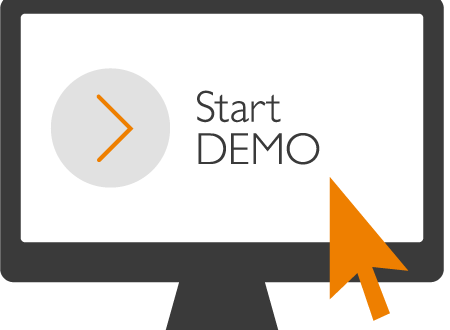
\includegraphics[width=0.85\textwidth]{Chapter1/demo1}
%  \caption{An illustration.}
%  \label{fig:demo1}
%\end{figure}

%
Deep learning, a sub-field of machine learning capable of learning higher-dimension feature representations via neural networks and gradient descent, has attracted remarkable attention from researchers over the last few decades.
%
Landmark works in deep learning, for example, the first attempt of using GPUs in training neural networks~\cite{krizhevsky2012imagenet}, the introduction of the self-supervised training technique capable of mapping words to representation space~\cite{mikolov2013efficient}, or the introduction of the Transformer architecture~\cite{vaswani2017attention}, have actively and significantly driven the deep learning research community forward. 
%
On the one hand, the ability to recognize patterns presented in and extract information from a large amount of data, without relying on handcrafting rules and heuristics, has made deep learning methods incredibly powerful and attractive.
%
On the other hand, countless applications of deep learning have been developed in many aspects of our lives, from vision tasks such as facial recognition~\cite{masi2018deep}, image restoration~\cite{gao2017demand}, natural language tasks such as machine translation~\cite{stahlberg2020neural}, speech recognition~\cite{kumar2019comprehensive}, to more complex decision-making tasks such as autonomous driving~\cite{kiran2021deep} or healthcare treatment administration~\cite{yu2021reinforcement}.

\section{Question Answering}
\label{sec:qa}

\begin{figure}[!htbp]
	\centering
	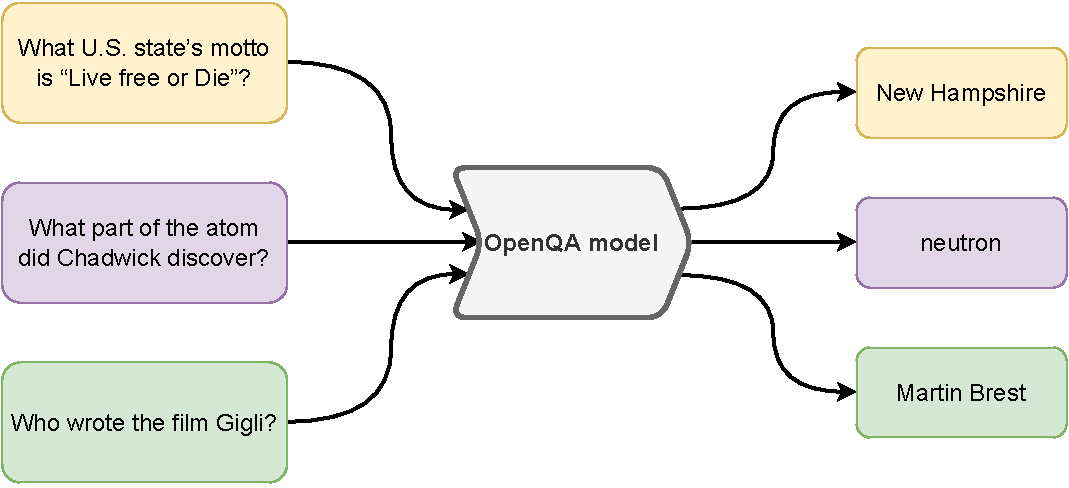
\includegraphics[width=0.7\linewidth]{introduction/openqa.pdf}
	\caption[Examples of input-output pairs in open-domain question answering.]{
		%
		Examples of input-output pairs in open-domain question answering (OpenQA).
		%
		The goal of OpenQA is to answer any factoid question about nearly anything. Adapted from~\cite{chen2020open}.
	}
	\label{fig:openqa}
\end{figure}


%
Question answering (QA), a naturally arisen task that aims at answering questions posed by humans, has generally received great attention thanks to the wide range of real-world applications that it offers.
%
However, most of the previous works on QA have mainly placed their focus on closed-domain question answering and machine reading comprehension (MRC).
%
While closed-domain QA limits the questions being asked to a specific domain knowledge (e.g., medicine), or to a specific type of questions (e.g., \emph{when}), MRC systems are allowed to read and comprehend relevant context passages in order to answer the questions.
%
In contrast, the long-standing problem of open-domain question answering~\cite{voorhees1999trec} (OpenQA) has observed significantly less progress, potentially due to its complex and large-scale nature.
%
Open-domain question answering is a much more challenging task than closed-domain QA or MRC as it requires cutting-edge techniques from both natural language processing (NLP) and information retrieval (IR).
%
In OpenQA, the model must answer any factoid questions, possibly about anything, without being provided relevant contexts containing the answer.
%
\fref{fig:openqa} illustrates several examples of input-output pairs in OpenQA.
%
Notably, OpenQA can be utilized in a wide range of applications, ranging from online customer service systems, chatbots (e.g., Siri) to search engines (e.g., Google), where user inputs are usually information-seeking questions.
%
With OpenQA, we aim at developing intelligent systems that automatically retrieve and extract relevant information of a given question, and subsequently suggest a detailed answer.

\section{Closed-book and Open-book Open-domain Question Answering}
\label{sec:close_and_open_book}

%
OpenQA can be further classified into two categories, namely closed-book OpenQA and open-book OpenQA.

\subsection{Closed-book Open-domain Question Answering}
\label{sec:close_book}
%
In closed-book OpenQA, the system is not given access to any textual documents when answering the questions, and thus is expected to memorize factual knowledge ahead of time stored implicitly in its parameters (\emph{parametric memory}).
%
At test time, the system is expected to provide answers to questions that it has already encountered during training by
retrieving from its memory, or to infer answers to unseen questions using general ontologies and common
knowledge.
%
This is analogous to a student memorizing possible question-answer pairs from a set of past year papers before coming to a closed-book final examination.

%
Despite its simplicity and straightforward formulation, there exists a number of inherent weaknesses in closed-book OpenQA systems.
%
First, closed-book OpenQA models, which are generative models by design, have been long known to suffer from \emph{factual hallucination}~\cite{ji2022survey}.
%
Factual hallucination is a common phenomenon in text generation in which the models fail to precisely retrieve factual information from their parametric memory, and thus unintendedly attempt to fabricate it.
%
Such unfaithful behaviors should obviously be avoided in question answering where precise fact is of utmost importance.
%
Second, closed-book OpenQA systems generally require a huge number of parameters to accommodate their parametric memory, which often far exceeds the amount of storage used to store factual knowledge in plain text.
%
For example, a state-of-the-art closed-book OpenQA system~\cite{roberts2020much} is only able to match the performance of a recent open-book OpenQA system~\cite{karpukhin2020dense} while requiring 11 times as many parameters.
%
Third, it is not trivial to update closed-book OpenQA models with new information (for example recent events), as it would require re-training the models.
%
This in turn gives rise to the \emph{catastrophic forgetting} problem~\cite{kemker2018measuring}, another common issue in deep learning in which the model loses its generalizability and catastrophically forgets existing knowledge after being trained on new data.

\subsection{Open-book Open-domain Question Answering}
\label{sec:open_book}
%
Open-book OpenQA has been proposed to tackle the aforementioned issues that closed-book OpenQA suffers from. 
%
At inference time, an open-book OpenQA system is provided access to a large knowledge base, for example Wikipedia articles, from which it can search for supporting passages to the given question.
%
This formulation allows the system to retrieve precise factual knowledge from the non-parametric memory of passages, effectively overcoming the factual hallucination and catastrophic forgetting problems.
%
At the same time, the number of parameters can be significantly reduced given that the models no longer have to memorize information by storing it in the parameters.
%
Finally, such non-parametric knowledge source as Wikipedia is human interpretable and can be easily updated.
%
Given these advantages, in this work, we mainly tackle the problem of open-book OpenQA and simply refer to it as~\emph{OpenQA}  for brevity.


\begin{figure}[!htbp]
	\centering
	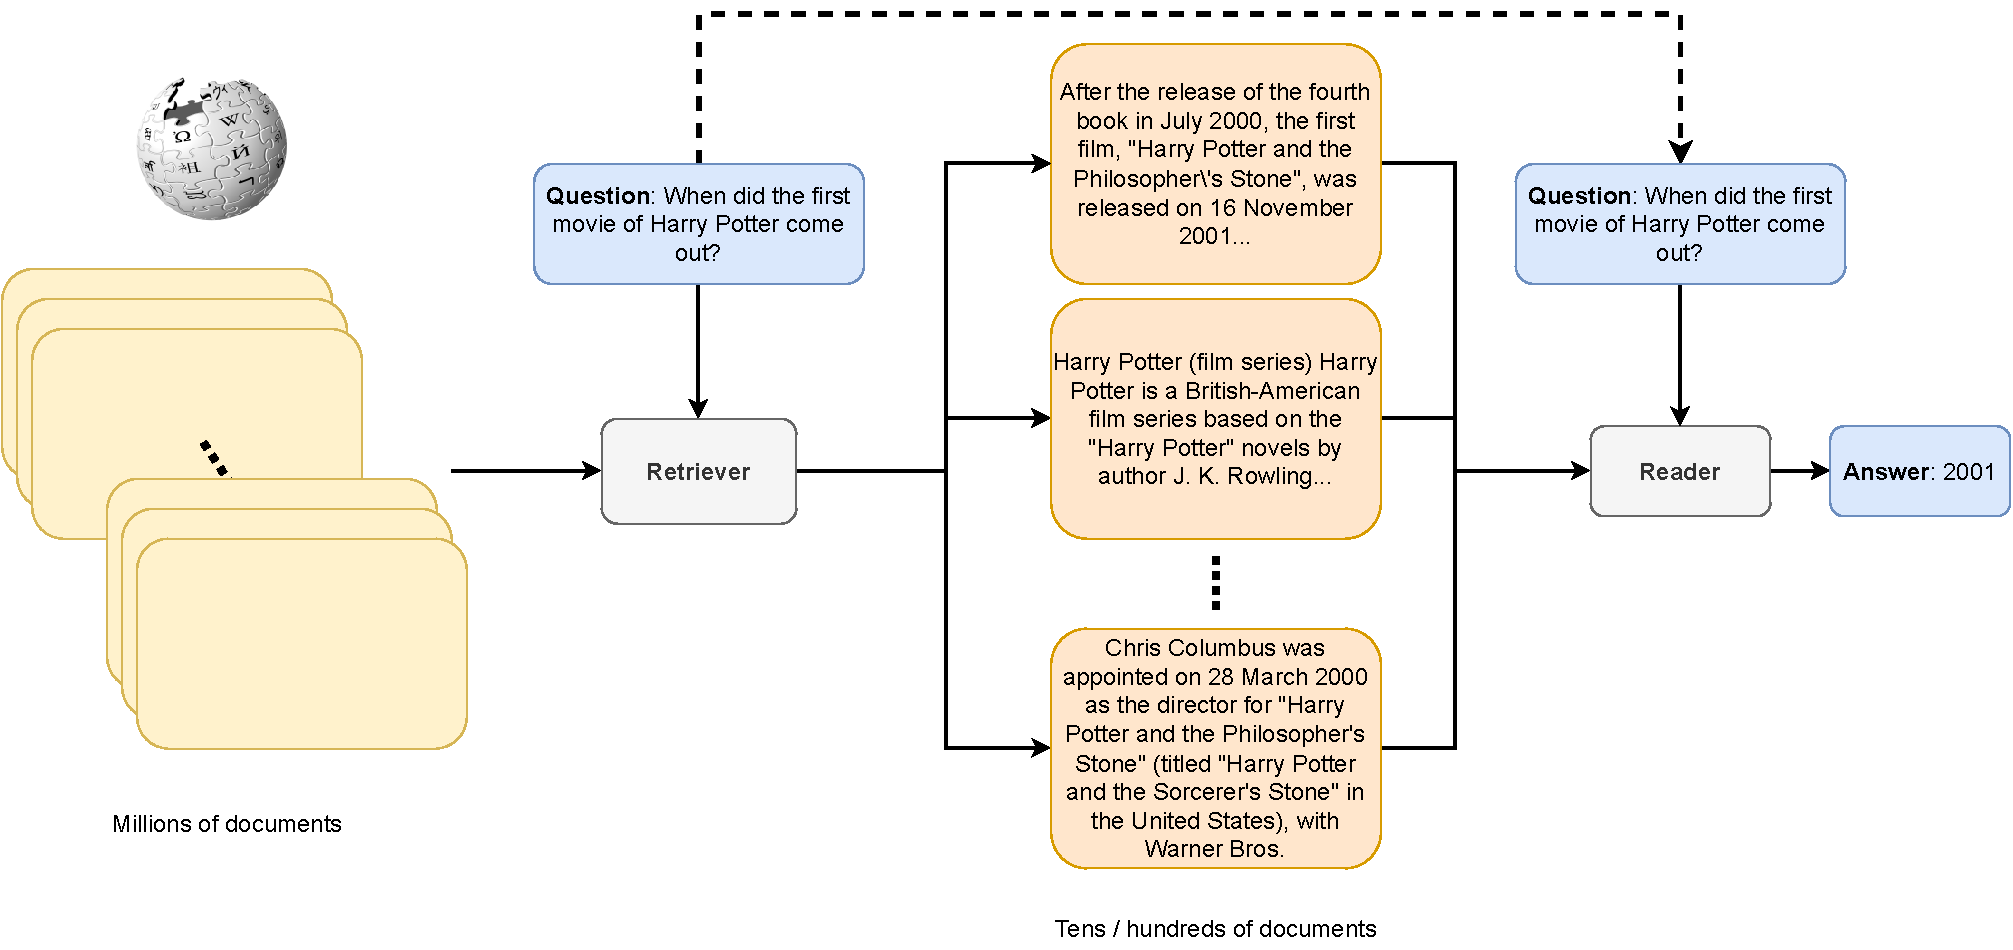
\includegraphics[width=0.95\linewidth]{introduction/open_book_openqa.pdf}
	\caption[An overview of the two-stage retriever-reader model.]{
		%
		An overview of the two-stage retriever-reader model.
		%
		The retriever first performs a highly efficient search algorithm to retrieve top-$k$ most relevant passages from a large collection of documents (e.g., Wikipedia).
		%
		The reader then reads this subset of documents to infer the answer to the given question.
	}
	\label{fig:open_book_openqa}
\end{figure}


%
It is important to highlight that we are processing millions of documents in open-book OpenQA given a single input query.
%
Thus, it would be computationally infeasible to naively apply machine reading comprehension to every passage in the corpus and return the most probable answer.
%
To overcome this challenge,~\citet{chen2017reading} proposed a two-stage~\emph{retriever-reader} paradigm that has gained popularity recently due to its effectiveness and efficiency.
%
\fref{fig:open_book_openqa} presents an overview of this approach.
%
In the first stage of this framework, a small number of relevant passages is retrieved by a \emph{retriever} model using a highly efficient search algorithm.
%
A~\emph{reader} model is then used to perform reading comprehension on this subset of passages to obtain the final answer.
%
Analogously, in an open-book exam, the students should first identify relevant sections in the
textbooks before actually delving into the details to find answers to a given question, instead
of reading every paragraph one by one looking for the solutions.

%
In~\citet{chen2017reading}, a simple TF-IDF~\cite{jones1972statistical} weighted bag-of-words method is used as the retrieval method while an LSTM-based~\cite{hochreiter1997long} model is employed as the MRC method.
%
The retrieval method, which belongs to a family of non-trainable~\emph{sparse retrieval} approaches, performs a simple and efficient word matching step to find relevant passages.
%
On the other hand, the reader model has a limited capability of understanding long sequences, be it the forgetfulness in RNN-based models or quadratic time complexity in Transformer-based models~\cite{devlin2019bert}.
%
Since the introduction of the two-stage paradigm, many advances in Natural Language Processing (NLP) have been proposed to push the boundary of OpenQA systems further, especially the retriever model.
%
\citet{lee2019latent} and~\citet{guu2020realm} adopted trainable~\emph{dense retrieval} models, which are first pre-trained in an unsupervised manner before being fine-tuned on the downstream OpenQA data.
%
\citet{seo2019real} combined the complementary advantages of sparse retrieval and dense retrieval in a unified framework.
%
\citet{khattab2020colbert} aimed to address a key challenge in dense retrieval, namely the \emph{decomposability gap} which we will introduce shortly, with vector decomposition and late interaction to mimic the self-attention~\cite{vaswani2017attention} mechanism.
%
Dense Passage Retrieval (DPR)~\cite{karpukhin2020dense} later showed that pre-training is not needed for dense retrieval as the retriever model directly trained on OpenQA data with in-batch negatives and the negative log-likelihood (NLL) objective function significantly outperformed all other approaches.

%
In all of the previous algorithms, the query and passage texts will first be compressed into some vectorized form in order to enable a highly efficient search algorithm on the retriever side.
%
For sparse retrieval, the documents are encoded with weighted word frequency, for which severe information loss will incur such as the loss of sequential information and semantic meaning of the texts.
%
On the other hand, for dense retrieval, information compression is done by mapping each sequence of words to its high-dimensional vector representation.
%
Not only does this approach benefit from the advantages of representation learning from supervised data, but it also enables the use of the well-studied, highly efficient Maximum Inner Product Search (MIPS)~\cite{johnson2019billion} algorithm.
%
Notably, regardless of the retrieval type, the computational cost of extracting information from the knowledge base can be further amortized by pre-computing and pre-indexing it into a MIPS index.
%
As a result, at test time, we only need to compress the input question (e.g., by feeding it through the dense retriever model to obtain its vector representation) before sending it to the MIPS index for efficient retrieval of relevant passages.
%
This procedure effectively reduces the number of passages for the reader model from millions of documents to 50-100 documents in real-time.
%
However, it also inevitably limits the ability of the model to capture mutual information between the passages and the input questions (so-called the \emph{decomposability gap}).
%
As discussed above, this is to some extent caused by the loss of information during the data compression step, even for dense retrievers.
%
Moreover, it is important to note that the evidence documents and the input query are encoded independently of each other.
%
Thus, the task of the retrievers is to find the best passage matches to a given question when both the passages and the question have already been encoded, without being allowed to comprehend the original texts.
%
In other words, decomposability gap happens when the computationally expensive reading comprehension task is decomposed into two smaller and efficient tasks of feature representation and maximum inner product search.
%
As a consequence, this performance trade-off significantly negatively affects the relevance of passages retrieved in the first stage, which in turn is detrimental to the reader performance, thus the overall OpenQA performance.

%
Decomposability gap is regarded as the most challenging yet attractive problem in OpenQA.
%
Previous work on mitigating this challenge can be classified into several main directions.
%
To explicitly tackle the decomposability gap, \citet{khattab2020colbert} aimed at mimicking the self-attention mechanism between the passage and the input query via late vector interaction, while~\citet{das2018multi} allowed communication between the retriever and reader to iteratively fine-tune the retrieval results.
%
Another research direction is query expansion, whereby the input query is first augmented with relevant keywords before compression, effectively pushing the representation of this query closer towards that of the gold passages in the feature representation space~\cite{mao2021generation, qi2019answering}.
%
Notably, a large body of works focused on improving the retriever performance with novel pre-training paradigms~\cite{lee2019latent, guu2020realm, lewis2020retrieval, chang2020pre, lewis2020pre, xiong2021progressively}.
%
Lastly,~\citet{seo2019real},~\citet{lee2020contextualized} and~\citet{luan2021sparse} combined the complementary strengths of sparse and dense retrieval to improve the overall retrieval performance.
%
In this final year project, we extend upon the outstanding work Dense Passage Retrieval~\cite{karpukhin2020dense}.
%
We explore the first three aforementioned directions as well as other directions and further propose multiple novel approaches with the main goal of improving the overall OpenQA performance, as well as with a particular focus on the decomposability gap of retrieval.



%%
%\citet{clark2018simple} as well as~\citet{wang2019multi} proposed several techniques to comprehend multiple passages simultaneously, thereby improving the reading comprehension performance while being more efficient.
%%
%Similarly,~\citet{wang2018evidence} proposed various methods to aggregate answers obtained from reading different passages, for example by their weighted frequency.
%%
%\citet{lee2019latent} pre-trained the retriever with Inverse Cloze Task and then jointly fine-tuned the retriever and the reader on OpenQA data.
%%
%\citet{guu2020realm} extended this direction by proposing a better pre-training paradigm called Salient Span Masking and a better joint training approach.
%%
%Dense Passage Retrieval (DPR) showed that 
%%
%\citet{lewis2020retrieval} combined both the pre-training and joint training paradigms 


%%
%This algorithm, which will be described later in more detail in~\FAKEREF{NEED REFERENCE!!}, is orders of magnitude faster than the naive approach, therefore enabling a real-time OpenQA performance.
%%
%However, this architectural design comes with an inherent trade-off, namely decomposability gap, which negatively affects the relevance in the returned documents.


%----------------------------------------------------------------------------------------
\section{Major Contributions}\label{sec:contribution}
Our main contributions can be stated as follows:
\begin{itemize}
\item
%
We propose several simple yet under-explored multi-task learning approaches for OpenQA that yield sizeable performance improvements while reducing the memory footprint of the retriever, which is critical for real-time OpenQA systems.

\item
%
We explore a simple method aimed at capturing the mutual information between the question query and documents during retrieval.
%
This method explicitly considers the decomposability gap and can be seen an alternative to the late interaction mechanism proposed in~\citet{khattab2020colbert}.

\item
%
We propose a simple data augmentation method to diversify the retrieval training data, thereby improving the previous state-of-the-art DPR retriever by a large margin.

\item
%
We investigate the effect of the objective function (so-called loss function) on retrieval training, from which we propose new objective functions for representation learning that achieve marginal gains over the baseline model.

\item
%
Finally, we propose a novel data synthesis - semi-supervised pre-training - query expansion paradigm with the goal of comprehensively improving both the retriever and reader, for which we achieve considerable performance improvements across several benchmarking datasets.


\end{itemize}


%\section{Outline of the Thesis}
%
%\FAKEREF{Work In Progress}

%\cref{ch:introduction} introduces ...
%
%\cref{ch:literature_review} reviews ...
%
%
%
%More chapters ....
%
%
%....


%\part{Part Name: Use it when there are many chapters}
%%!TEX root=../mythesis.tex
% Chapter Template

\chapter{Literature Review} % Main chapter title
\chaptermark{Literature Review}  % replace the chapter name with its abbreviated form
\label{ch:literature_review} % Change X to a consecutive number; for referencing this chapter elsewhere, use \ref{ChapterX}

\FAKEREF{Work In Progress}

%\lhead{Chapter X. \emph{Chapter Title Here}} % Change X to a consecutive number; this is for the header on each page - perhaps a shortened title
%-----------------------------------
% SECTION 1
%-----------------------------------

%\section{Part 1}
%
%When you cite a paper \cite{bauschke2011convex}, the back reference from bibgraph will apper as page number.
%
%You can also cite paper with author name using the command `citet': such as: \citet{bauschke2011convex}.
%
%\section{Part 2}
%
%cite another paper \cite{DynamicOptim_Opportunities_challenges}.
%
%\begin{lemma}[My lemma]
%	A great lemma.
%	\begin{equation}
%		c^2=a^2+b^2
%	\end{equation}
%\end{lemma}
%
%\begin{theorem}[My theorem]
%	A great theorem.
%	\begin{equation}
%		c^2=a^2+b^2
%	\end{equation}
%\end{theorem}
%
%\begin{proof}
%	The proof is intuitive.
%\end{proof}
%
%\begin{corollary}[My corollary]
%	A great corollary.
%	\begin{equation}
%		c^2=a^2+b^2
%	\end{equation}
%\end{corollary}
%
%\begin{proposition}[My proposition]
%	A great proposition.
%	\begin{equation}
%		c^2=a^2+b^2
%	\end{equation}
%\end{proposition}
%
%\begin{example}[My example]
%	A great example.
%	\begin{equation}
%		c^2=a^2+b^2
%	\end{equation}
%\end{example}
%
%\begin{definition}[My definition]
%	A great definition.
%	\begin{equation}
%		c^2=a^2+b^2
%	\end{equation}
%\end{definition}
%
%\begin{assumption}[My assumption]
%	A great assumption.
%	\begin{equation}
%		c^2=a^2+b^2
%	\end{equation}
%\end{assumption}
%
%\begin{remark}[My remark]
%	A great remark.
%	\begin{equation}
%		c^2=a^2+b^2
%	\end{equation}
%\end{remark}

%!TEX root=../mythesis.tex
% Chapter Template

\chapter{Background} % Main chapter title
\chaptermark{Background}  % replace the chapter name with its abbreviated form
\label{ch:background}


In this chapter, we present background that will be necessary to elaborate on our proposed approaches later in the report.
%
First, we introduce a typical experimental setup of OpenQA along with notations that we will be using throughout the report.
%
Next, we introduce Dense Passage Retrieval (DPR)~\cite{karpukhin2020dense}, a recently published work with a novel retriever training method with the negative log-likelihood objective function and in-batch negative technique.
%
We then describe the default experimental settings used in our experiments.
%
%We then review Fusion-in-Decoder (FiD)~\cite{izacard2021leveraging}, a novel generative reader model capable of reading and aggregating information from hundreds of documents to produce answers.



\section{Notations}\label{sec:notations}
%
For OpenQA, we are given a large corpus of documents containing factual information from which we retrieve knowledge needed to perform question answering.
%
It is a common practice in the OpenQA literature to split each of these documents into several text chunks of equal lengths~\cite{karpukhin2020dense, wang2019multi, lewis2020retrieval, xiong2020approximate, fajcik2021pruning, izacard2020distilling, izacard2021leveraging}, resulting in a corpus $\mathcal{C}$ of $M$ passages $\mathcal{C} = \{p_1, p_2, \ldots, p_M\}$.
%
This is because existing reading comprehension methods have a limited capability of reading long sequences as discussed in~\sref{sec:open_book}.
%
Each passage $p_i$ can further be viewed as a sequence of tokens (words) $w_1^{(i)}, w_2^{(i)}, \ldots, w_{\vert p_i \vert}^{(i)}$.
%
Given an input question $q$, the task is to find its answer under the form of a text span $w_{s, e}^{(i)} = w_s^{(i)}, w_{s + 1}^{(i)}, \ldots, w_e^{(i)}$ of a passage $p_i$, where $s$ and $e$ denote the~\emph{start} and~\emph{end} indices of the span, respectively.
%
It is important to highlight the flexibility of OpenQA that during inference, any text corpus can be used to answer the question as long as it provides necessary information.
%
In practice, the corpus size can range from millions (e.g., Wikipedia) to billions or trillions (e.g., the Web) of passages.

%
Under the two-stage retriever-reader paradigm, we have a retriever $R$ and a reader $S$ formulated as
%
\begin{definition}[Retriever]
	A retriever under the two-stage paradigm is a model that returns a small filtered subset of the given large set of passages.
	\begin{equation}
	R(q, \mathcal{C}) = \mathcal{C_F}
	\end{equation}
\end{definition}
%
\begin{definition}[Reader]
	A reader under the two-stage paradigm is a model that produces an answer to the given question given the filtered set from the retriever.
	\begin{equation}
	S(q, \mathcal{C_F}) = w_{s, e}^{(i)}
	\end{equation}
\end{definition}
%
where $\mathcal{C_F}$ is a small set of $k$ passages with $k \ll M$ and $w_{s, e}^{(i)}$ is the final answer of the OpenQA system to the question $q$.
%
In other words, the task of the retriever is to efficiently retrieve a small set $\mathcal{C_F}$ of passages that it considers relevant.
%
The reader will then carefully comprehend the question $q$ as well as each of the passages in $\mathcal{C_F}$ to infer the answer.
%
We refer readers to~\fref{fig:open_book_openqa} for an illustration of an OpenQA system.

Furthermore, throughout this report, we refer to an~\emph{encoder}, denoted as $E$, as a BERT model~\cite{devlin2019bert} that first appends a special token \texttt{[CLS]} to the input text sequence and then maps the sequence to the embedding of \texttt{[CLS]}.
\begin{definition}[Encoder]
	An encoder is a model that maps an input text sequence
	\begin{align*}
	p = \{\texttt{[CLS]}, w_1, w_2, \ldots, w_{\vert p \vert}\}
	\end{align*}
	to the vector embedding of the special token token $\texttt{[CLS]}$
	\begin{equation}
	E(p)_{\texttt{[CLS]}} = \mathbf{v}_{\texttt{[CLS]}} \in \mathbb{R}^{d}
	\end{equation}
\end{definition}
%
where $d$ is the embedding dimension, and $\mathbf{v}_{\texttt{[CLS]}}$ is known as the feature representation~\footnote{In this report we will use~\emph{embedding},~\emph{feature} and~\emph{representation} interchangeably.} of the special token \texttt{[CLS]}.
%
Historically, \texttt{[CLS]} is appended to the input to serve as a contextualized embedding that encodes the semantic meaning of the \emph{entire} sequence~\cite{devlin2019bert}.
%
With a proper objective function, we can train $E$ to encode important semantic meaning of $p$ into $\mathbf{v}_{\texttt{[CLS]}}$.




\section{DPR Retriever}
\label{sec:dpr_retriever}


\begin{figure}[!htbp]
	\centering
	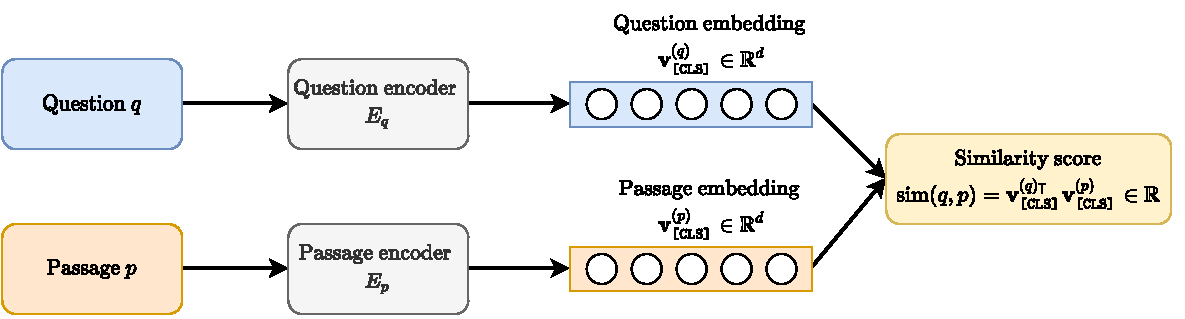
\includegraphics[width=0.9\linewidth]{background/two_tower.pdf}
	\caption[Two-tower architecture of DPR retriever.]{
		%
		The two-tower architecture of the DPR retriever, consisting of a question encoder and a passage encoder.
		%
		Each of the towers encodes input texts into their embedding vectors, and the final similarity score is computed as their dot product.
		%
		Adapted from~\cite{chen2020open}.
	}
	\label{fig:two_tower}
\end{figure}


%
Despite its simplicity, DPR was able to outperform all prior arts by large margins when it was introduced.
%
In this section, we describe the retriever component of DPR and refer interested readers to~\cite{karpukhin2020dense} for a detailed description of the reader component.
%
The DPR retriever consists of a passage encoder $E_P$ and a question encoder $E_Q$, whose task is to embed passages and questions to their representation space, respectively.
%
\begin{equation}
	\label{eq:dpr_encode}
	\begin{split}
	E_P(p)_{\texttt{[CLS]}} = \mathbf{v}^{(p)}_{\texttt{[CLS]}} \in \mathbb{R}^d \\ 
	E_Q(q)_{\texttt{[CLS]}} = \mathbf{v}^{(q)}_{\texttt{[CLS]}} \in \mathbb{R}^d
	\end{split}
\end{equation}
%
We then define the similarity between a question and a passage as their dot product.
\begin{definition}[Vector similarity]
	\label{def:sim}
	The similarity between a question and a passage is defined as the dot product of their vector embeddings.
	\begin{equation}
	\label{eq:sim_score}
	\text{sim}(q, p) = \mathbf{v}^{(q)\intercal}_{\texttt{[CLS]}} \mathbf{v}^{(p)}_{\texttt{[CLS]}} \in \mathbb{R}
	\end{equation}
\end{definition}
%
\fref{fig:two_tower} presents an illustration of the DPR retriever.
%
This two-tower architecture is widely used in~\emph{metric learning}~\cite{han2015matchnet, song2019occlusion} and~\emph{self-supervised learning}~\cite{zbontar2021barlow, mitrovic2020representation} in which models are trained to maximize the similarity of similar inputs and minimize the similarity of dissimilar inputs.
%
As discussed in~\sref{sec:open_book}, this design brings about the real-time performance of the well-studied Maximum Inner Product Search (MIPS) algorithm~\cite{johnson2019billion} but at the same time is detrimental to the retrieval performance due to the decomposability gap which we aim to address.

%
In this project, we follow the DPR implementation and use BERT~\cite{devlin2019bert} as the architecture for all encoders.
%
As a result, each embedding vector is a $d=768$-dimensional vector.
%
We omit the details of BERT and refer interested readers to~\cite{devlin2019bert}.

%
\subsection{Training and Inference}
\label{sec:dpr_training}
%
Given an input question $q_i$ posed by users, we denote $p^{+}_i$ as a positive passage that contains an answer to $q_i$, and $p^{-}_i$ as a negative passage otherwise.
%
Intuitively, we want to train the model to maximize the similarity between $q_i$ and $p^{+}_i$, at the same time minimizing the similarity between $q_i$ and $p^{-}_i$.
%
Formally, under the metric learning framework, we want to construct an \emph{latent space} such that relevant pairs of questions and passages are closer to each other than irrelevant pairs.
%
Therefore, given a question $q_i$, a relevant passage $p^{+}_i$ and a set of $n$ irrelevant passages $\{p^{-}_{i, 1}, p^{-}_{i, 2}, \ldots, p^{-}_{i, n}\}$, we train the model to minimize the negative log-likelihood loss function:
%
\begin{definition}[Negative log-likelihood]
	\label{def:nll}
	The negative log-likelihood loss function of the positive passages.
	\begin{equation}
	L(q_i, p^{+}_i, p^{-}_{i, 1}, p^{-}_{i, 2}, \ldots, p^{-}_{i, n}) = - \log \frac{e^{\text{sim}(q_i, p^{+}_i)}}{e^{\text{sim}(q_i, p^{+}_i)} + \sum_{j = 1}^{n} e^{\text{sim}(q_i, p^{-}_{i, j})}}
	\end{equation}
\end{definition}
%
where we apply the softmax function to the similarity vector before taking its negative log value.
\begin{definition}[Softmax]
	\label{def:softmax}
	Softmax is the function that takes as input a vector of $K$ real numbers and outputs a normalized probability distribution vector of the same length.
	\begin{equation}
	\sigma(\mathbf{z})_i = \frac{e^{z_i}}{\sum_{j = 1}^{K}e^{z_j}} \text{ for } i = 1, 2, \ldots, K
	\end{equation}
\end{definition}
%
In practice, we consider passages to be positive if they contain a text span that matches the answer of the question, and negative otherwise.

%
In addition to the simple yet novel negative log-likelihood objective function,~\citet{karpukhin2020dense} also proposed a simple in-batch negative training setting that works extremely well empirically.
%
Suppose we have a mini-batch of $B$ (question, positive passage) pairs.
%
We first feed this batch through the two-tower retriever to obtain a question embedding matrix $\mathbf{Q} \in \mathbb{R}^{B \times d}$ and a passage embedding matrix $\mathbf{P} \in \mathbb{R}^{B \times d}$.
%
The similarity matrix is then computed as:
%
\begin{equation}
\mathbf{S} = \mathbf{Q}\mathbf{P}^\intercal \in \mathbb{R}^{B \times B}
\end{equation}
%
By doing so, we are effectively comparing $B^2$ question-passage pairs in the mini-batch, from which we want to minimize the negative log of the softmaxed values along the diagonal of the square similarity matrix $\mathbf{S}$.
%
This is called~\emph{in-batch negatives} since we reuse computations from within the batch with positive passages of other questions as negative passages, thereby efficiently reducing the memory footprint and effectively scaling the batch size up.
%
Furthermore,~\citet{karpukhin2020dense} proposed to utilize an additional hard negative passage per each question in the minibatch, obtained from the sparse retrieval method BM25~\cite{robertson2009probabilistic}.
%
In other words, each question will be associated with a single positive passage and $2B - 1$ negative passages, of which $2(B - 1)$ passages are in-batch negatives and one passage is hard negative.

%
During inference, we first build a FAISS index~\cite{johnson2019billion} by feeding all available passages in the corpus to $E_P$.
%
This incurs a non-recurring cost since this step is only done once.
%
At run-time, given an input question $q$, we obtain its embedding via $\mathbf{v}^{(q)}_{\texttt{[CLS]}} = E_Q(q)_{\texttt{[CLS]}}$, which gets sent to the FAISS index to perform top-$k$ similarity search.
%
A set $\mathcal{C_F}$ of top-$k$ most relevant passages according to the similarity score $\text{sim}(q, p_i)$ is produced by the algorithm in milliseconds, concluding the retrieval step.



\section{Experimental Setup}\label{sec:exp_setup}
%
In this section we briefly describe the default experimental setup used in our experiments.
%
We note that we reuse a substantial portion of the code and data given by the DPR authors~\footnote{https://github.com/facebookresearch/DPR/}~\cite{karpukhin2020dense}, unless otherwise specified below.
%
Therefore, we refer interested readers to~\cite{karpukhin2020dense} for further details on the setup.

\subsection{Data}\label{sec:exp_data}
%
Following~\cite{karpukhin2020dense}, we use the English Wikipedia dump from Dec. 20, 2018 as the knowledge source from which passage retrieval is done.
%
This knowledge base is provided by the DPR authors after post-processed to remove semi-structured data and split into chunks of 100-word passages.
%
There are in total 21,015,324 passages in this corpus.
%
On the other hand, we use Natural Questions (NQ)~\cite{kwiatkowski2019natural} as the question answering dataset on which we train and evaluate our retriever and reader models.
%
This dataset provides questions mined from the real Google search queries as well as the corresponding positive Wikipedia passages along with the answer text span.

\subsection{Evaluation Metrics}
%
Following~\cite{karpukhin2020dense}, we evaluate the retriever model by the~\emph{retrieval accuracy} and the reader model with~\emph{exact match (EM)} and~\emph{F1 score}.
%
Specifically, retrieval accuracy, or retrieval recall, is measured as the percentage of top-$k$ retrieved passages that contain the gold answer obtained from NQ.
%
It can be understood as how relevant your retrieved passages are to a given question.
%
On the reader side, exact match is a direct measure of the reader model performance.
%
It is calculated as the percentage of answers returned by the reader model that precisely match with one of the gold answers.
%
F1 score on the other hand allows some relexations on the returned answers by measuring the F1 score between the answer by the reader model and the gold answer.
%
\begin{definition}[F1 score]
	F1 score in the context of QA is calculated as the harmonic mean between the precision and recall of the returned answer and the gold answer.
	\begin{equation}
	\label{eq:f1_score}
	F_1 = \frac{2}{\text{recall}^{-1} + \text{precision}^{-1}}
	\end{equation}
\end{definition}
%\part{Again for Second Part}
%!TEX root=../mythesis.tex
% Chapter Template

\chapter{Shared Encoders} % Main chapter title
\chaptermark{Shared Encoders}  % replace the chapter name with its abbreviated form
\label{ch:shared_encoders}


\section{Method}\label{sec:shared_encoders_methods}


\begin{figure}[!htbp]
	\centering
	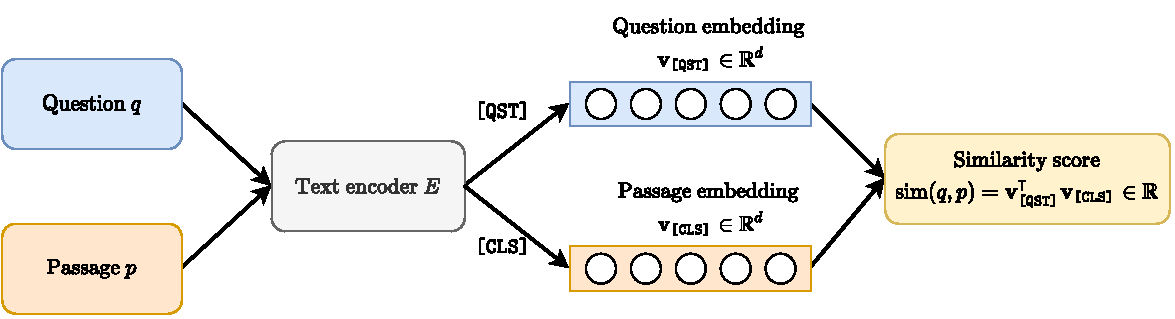
\includegraphics[width=0.9\linewidth]{shared_encoders/two_tower_shared.pdf}
	\caption[Two-tower architecture of DPR retriever with parameter sharing.]{
		%
		The two-tower architecture of the DPR retriever with parameter sharing.
		%
		The same encoder will encode input texts into their embedding vectors with proper special tokens \texttt{[QST]} or \texttt{[CLS]} to distinguish the input types.
	}
	\label{fig:two_tower_shared}
\end{figure}


%
In this chapter, we present our first contribution to the DPR architecture~\cite{karpukhin2020dense} -~\emph{shared encoders}.
%
Recall that the two-tower DPR retriever consists of a question encoder $E_Q$ and a passage encoder $E_P$ with the same architecture (i.e., BERT~\cite{devlin2019bert}) but different weights~\footnote{In the context of deep learning,~\emph{weights} refers to the values of the parameters of the model.}.
%
In this setup, the task of both encoders is to textual data to the same embedding space, one being question texts and one being passage texts.
%
Therefore, it emerges naturally that sharing parameters of these two models could be beneficial.

%
More specifically, we use the same set of parameters for the two encoders while assigning the special token \texttt{[CLS]} to the passage encoder and \texttt{[QST]} to the question encoder.
%
The similarity score between a question $q$ and a passage $p$ defined in~\eqref{eq:sim_score} then becomes:
%
\begin{equation}
\text{sim}(q, p) = \mathbf{v}^\intercal_{\texttt{[QST]}} \mathbf{v}_{\texttt{[CLS]}} \in \mathbb{R}
\end{equation}
%
~\fref{fig:two_tower_shared} illustrates the architectural design of this approach.
%
Under this architecture, we allow the models to share the general world knowledge and natural language understanding capabilities and at the same time to distinguish the input types.
%
Furthermore, this approach can be seen as a multi-task training algorithm, in which the general encoder $E$ is trained to map both questions and passages to the same feature space.


\section{Experimental Results}\label{sec:shared_encoders_results}


\begin{table*}[t!]
	\setlength\tabcolsep{5pt}
	\centering
	\small
	\begin{tabular}{ll|cccc}
		\toprule
		\textbf{Negative type} & \textbf{Retriever}
		& Top-1 & Top-5 & Top-20 & Top-100 \\ 
		\midrule
		\multirow{2}{*}{BM25} & DPR & 42.01 & 64.54 & 76.48 & 84.29 \\
		&DPR (shared encoders) & \textbf{45.01} & \textbf{66.70} & \textbf{78.25} & \textbf{85.62} \\
		\midrule
		\multirow{2}{*}{DPR hard negatives} & DPR & 49.36 & 67.34 & 78.09 & 85.40 \\
		& DPR (shared encoders) & \textbf{53.02} & \textbf{71.30} & \textbf{80.89} & \textbf{86.93} \\
		\bottomrule
	\end{tabular}
	\caption[Top-$\{1, 5, 20, 100\}$ retrieval accuracy on the Natural Questions test set of the DPR retriever with and without parameter sharing.]{
		%
		Top-$\{1, 5, 20, 100\}$ retrieval accuracy on the Natural Questions test set, calculated as the percentage of top-$k$ retrieved passages that contain the answer.
		%
		We present the results on training with two different negative types, BM25 or hard negatives.
		%
		The proposed shared encoders approach consistently and substantially outperforms the baseline DPR model on various settings with no additional cost.	
}
	
	\label{tab:shared_encoders_results}
\end{table*}


We provide the retrieval results on NQ in~\tref{tab:shared_encoders_results}, where we train the DPR model with BM25 hard negative passages described in~\sref{sec:dpr_training} and DPR hard negative passages, respectively.
%
In the latter case, negative passages are obtained by performing retrieval with a DPR checkpoint then for each question taking the highest-scoring passage that does not contain the answer.
%
We note that our results on the original DPR architecture do not match those reported in the original paper~\cite{karpukhin2020dense}, as we trained all these models with a batch size of 24 instead of 128 given our computation budget.
%
Nevertheless, we observe a consistent and considerable improvement of the shared encoders across different training settings and different top-$k$ evaluation.
%
This attests to our hypothesis earlier that this approach allows knowledge sharing and multi-task training that are beneficial to the model performance.

%
Intriguingly, we observe that the improvement of the shared encoders over the DPR baseline is consistently higher with DPR hard negatives than BM25 hard negatives.
%
For example, for top-5 retrieval accuracy, the performance gain of DPR shared encoders with DPR hard negatives is 3.96 points which is almost double of that with BM25 hard negatives (2.16 points).
%
This is opposite to the general intuition that it becomes increasingly difficult to improve a model when its performance is increased.
%
We hypothesize that this attributes to the knowledge sharing power of shared encoders, which can capitalize more on such informative negatives as DPR hard negatives.

%
Additionally, we note that by sharing the parameters of the two encoders, we effectively reduce the memory footprint by half.
%
This is especially critical in retrieval training where in-batch negatives are used, hence gradient accumulation is not sufficient to accommodate for a smaller batch size.
%
We expect the shared encoders to outperform the baseline DPR model even further when trained on a larger batch size, which is an advantage of shared encoders brought about by the memory efficiency of the architectural design.
%
We leave it to a future work to empirically verify this hypothesis.

%
Finally, we note that given its efficiency and effectiveness, we treat the DPR retriever with shared encoders as the baseline DPR model for all subsequent experiments, unless otherwise noted.
%!TEX root=../mythesis.tex
% Chapter Template

\chapter{Late Interaction} % Main chapter title
\chaptermark{Late Interaction}  % replace the chapter name with its abbreviated form
\label{ch:late_interaction}


\section{Method}
\label{ch:late_interaction_method}
%
In this chapter, we present our next contribution designed specifically to tackle the long-standing decomposability gap problem described in~\sref{sec:open_book}.
%
Recall that in the original DPR architecture, the question $q$ and passage $p$ are encoded \emph{independently} at run time (see~\eqref{eq:dpr_encode}), which later gets multiplied to obtain the dot product as their similarity score.
%
By doing so, we effectively decompose the task of reading both $q$ and $p$ together to the task of extracting important information from each $q$ and $p$ to embedding vectors and later comparing them.
%
Our goal is to minimize the information loss caused by the extraction step.


\begin{figure}[!htbp]
	\centering
	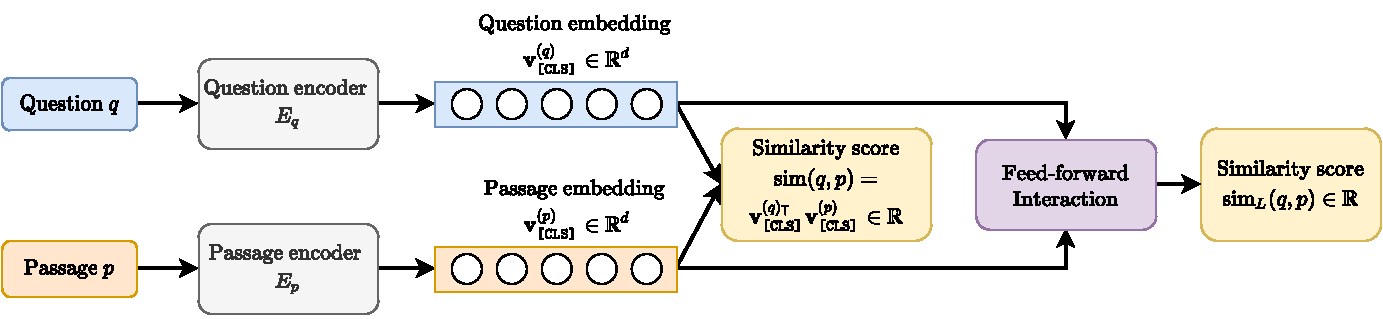
\includegraphics[width=1.0\linewidth]{late_interaction/two_tower_late_interaction.pdf}
	\caption[Two-tower architecture of DPR retriever with the late interaction mechanism.]{
		%
		The two-tower architecture of the DPR retriever with the late interaction mechanism.
		%
		After the top-$n$ retrieval with the usual similarity scores $\text{sim}(q, p)$, where $n > k$, embedding vectors are fed to the feed-forward interaction layer to obtain the late interaction similarity scores $\text{sim}_L(q, p)$, after which the final set of ranked passages is returned.
	}
	\label{fig:two_tower}
\end{figure}


%
In this work, we propose to append a small parametric module after the information extraction step.
%
This component is designed to \emph{recover} necessary information from both the question and passage embeddings that will then be compared again for retrieval, thus called \emph{late interaction}.
%
\fref{fig:two_tower} presents an overview of our proposed method.
%
Specifically, suppose we have a question embedding vector $\mathbf{v}^{(q)}_{\texttt{[CLS]}} \in \mathbb{R}^d$ and a passage embedding vector $\mathbf{v}^{(p)}_{\texttt{[CLS]}} \in \mathbb{R}^d$ obtained from the question encoder and passage encoder, respectively, using~\eqref{eq:dpr_encode}.
%
We then allows simple interactions between the two vectors
%
\begin{equation}
\label{eq:late_concat}
\mathbf{v}^{(qp)}_{\texttt{[CLS]}} = [\mathbf{v}^{(q)}_{\texttt{[CLS]}}; \mathbf{v}^{(p)}_{\texttt{[CLS]}}; \mathbf{v}^{(q)}_{\texttt{[CLS]}} \odot \mathbf{v}^{(p)}_{\texttt{[CLS]}}; \mathbf{v}^{(q)}_{\texttt{[CLS]}} - \mathbf{v}^{(p)}_{\texttt{[CLS]}}] \in \mathbb{R}^{4d}
\end{equation}
where $[\cdot;\cdot]$ denotes vector concatenation and $\odot$ denotes the Hadamard product, which is a element-wise operation.
%
We obtain $\mathbf{v}^{(qp)}_{\texttt{[CLS]}}$, a vector containing information when the question representation is allowed to interact with the passage representation on the feature level via element-wise arithmetic operations.
%
This information-rich vector is then fed through a simple feed-forward (FFN) parametric module to obtain the final similarity score
\begin{equation}
\label{eq:late_sim}
\text{sim}_L(q, p) = \mathbf{m}_L^\intercal \mathbf{v}^{(qp)}_{\texttt{[CLS]}}  \in \mathbb{R}
\end{equation}
%
where $\mathbf{m}_L \in \mathbb{R}^{4d}$ is the weight vector of the FFN.

During training, we apply the same negative log-likehood objective function defined in Definition~\ref{def:nll} to the novel late interaction similarity scores
%
\begin{equation}
L_L(q_i, p^{+}_i, p^{-}_{i, 1}, p^{-}_{i, 2}, \ldots, p^{-}_{i, n}) = - \log \frac{e^{\text{sim}_L(q_i, p^{+}_i)}}{e^{\text{sim}_L(q_i, p^{+}_i)} + \sum_{j = 1}^{n} e^{\text{sim}_L(q_i, p^{-}_{i, j})}}
\end{equation}
%
The final objective function is then taken as sum of the two individual losses
\begin{equation}
L_{\text{late\_interaction}} = L(q_i, p^{+}_i, p^{-}_{i, 1}, p^{-}_{i, 2}, \ldots, p^{-}_{i, n}) + \lambda L_L(q_i, p^{+}_i, p^{-}_{i, 1}, p^{-}_{i, 2}, \ldots, p^{-}_{i, n})
\end{equation}
%
where $\lambda$ is the weight of the late interaction objective component.
%
In other words, we train the retriever model to minimize the losses with respect to both the usual similarity scores and late-interaction similarity scores, which can also be viewed as a multi-task training paradigm.

%
At test time, we use $\text{sim}(q, p)$ for our retrieval method and $\text{sim}_L(q, p)$ for our re-ranking method.
%
In particular, given at input query $q$, we first retrieve a set $\mathcal{C_F}\prime$ of top-$n$ highest-scoring passages from a pre-built FAISS index as described in~\sref{sec:dpr_training}, where $n > k$.
%
This means that we retrieve more passages than we need.
%
Afterwards, we feed the question feature embeddings $\mathbf{v}^{(q)}_{\texttt{[CLS]}}$ as well as the embeddings of each passage in $\mathcal{C_F}\prime$ to the late interaction module via~\eqref{eq:late_concat} and~\eqref{eq:late_sim} to obtain the late-interaction similarity scores with minimal additional computational cost.
%
These scores are then used to re-rank and filter the passages in $\mathcal{C_F}\prime$ to obtain the final set $\mathcal{C_F}$ of $k$ most relevant passages.


\section{Experimental Results}
\label{ch:late_interaction_results}


\begin{table*}[t!]
	\setlength\tabcolsep{5pt}
	\centering
	\small
	\begin{tabular}{ll|cccc}
		\toprule
		\textbf{Architecture} & \textbf{Loss function}
		& Top-1 & Top-5 & Top-20 & Top-100 \\ 
		\midrule
		\multirow{2}{*}{\shortstack{DPR \\(shared encoders)}} &
		DPR loss & \textbf{53.02} & \textbf{71.30} & \textbf{80.89} & \textbf{86.93} \\
		& DPR loss + late interaction loss & 51.66 & 69.42 & 79.64 & 86.15 \\
		\bottomrule
	\end{tabular}
	\caption[Top-$\{1, 5, 20, 100\}$ retrieval accuracy on the Natural Questions test set of the DPR retriever (shared encoders) with and without the late interaction module.]{
		%
		Top-$\{1, 5, 20, 100\}$ retrieval accuracy on the Natural Questions test set of the DPR retriever (shared encoders) with and without the late interaction module, calculated as the percentage of top-$k$ retrieved passages that contain the answer.
		%
		The proposed interaction component degrades the baseline DPR model performance by a sizable margin.
	}
	
	\label{tab:shared_encoders_results}
\end{table*}


%
We conduct an experiment on NQ following the experimental settings described in~\sref{sec:exp_setup} with a batch size of 24.
%
The baseline model is taken as the DPR retriever with parameter sharing introduced in~\cref{ch:shared_encoders}, and the hyperparameters are set to $\{n, \lambda\} = \{200, 1.0\}$.
%
\tref{tab:shared_encoders_results} presents the retrieval recall on the NQ test set.

%
We observe that the late interaction component brings about a marginal performance loss to the DPR retriever.
%
We believe there are several reasons that make designing a late interaction layer difficult.
%
First, the proposed interaction layer consists of a small parametric module with weights $\mathbf{m}_L \in \mathbb{R}^{4d}$, which might not be sufficient to fully capture such complex natural language interactions.
%
Second, our interaction layer makes use of only element-wise operations (\eqref{eq:late_concat}), therefore is incapable of modeling the complex cross-feature interactions between the question embeddings and passage embeddings.
%
Lastly, it is worth noting that we did not specifically tune the newly introduced hyperparameters $\{n, \lambda\}$ which can have a huge impact on the final model performance.
%
Nevertheless, a concurrent work of~\citet{khattab2020colbert} that shares a very similar idea to our proposed late interaction has shown that this mechanism is a valuable addon to the existing retriever to combat the problem of decomposability gap.
%
Therefore, we refer interested readers to~\cite{khattab2020colbert} for a complete work on this idea.

%!TEX root=../mythesis.tex
% Chapter Template

\chapter{Multi-similarity Loss} % Main chapter title
\chaptermark{Multi-similarity Loss}  % replace the chapter name with its abbreviated form
\label{ch:multi_similarity}


\section{Method}
\label{sec:multi_similarity_method}


%
In this chapter, we introduce our novel multi-similarity loss for the DPR retriever model.
%
Recall that~\citet{karpukhin2020dense} proposed a negative log-likelihood (NLL) objective function that aimed to maximize the similarity between relevant question-passage pairs while minimizing the similarity of the irrelevant ones, as formulated in Definition~\ref{def:nll}
%
\begin{equation}
\label{eq:nll}
L(q_i, p^{+}_i, p^{-}_{i, 1}, p^{-}_{i, 2}, \ldots, p^{-}_{i, n}) = - \log \frac{e^{\text{sim}(q_i, p^{+}_i)}}{e^{\text{sim}(q_i, p^{+}_i)} + \sum_{j = 1}^{n} e^{\text{sim}(q_i, p^{-}_{i, j})}}
\end{equation}
%
On top of that,~\citet{karpukhin2020dense} proposed the in-batch negative mechanism to take advantage of the computation used in extracting features from other passages within the same batch.
%
Under the in-batch negative settings where we have a batch of $B$ samples, in which each question $q_i$ is associated with one positive passage $p^{+}_i$ and one hard negative passage $p^{-}_i$.
%
We rewrite the question-passage loss function in~\eqref{eq:nll}  with respect to a single sample at index $i$ as
%
\begin{equation}
\label{eq:nll_rewritten}
L^{qp}_i = - \log \frac{e^{\text{sim}(q_i, p^{+}_i)}}{
	\underbrace{
		\vphantom{\sum_{\substack{j = 1 \\ j \neq i}}^{B} e^{\text{sim}(q_i, p^{+}_j)}}
		e^{\text{sim}(q_i, p^{+}_i)}
	}_{\text{positive}} +
	\underbrace{
		\vphantom{\sum_{\substack{j = 1 \\ j \neq i}}^{B} e^{\text{sim}(q_i, p^{+}_j)}}
		e^{\text{sim}(q_i, p^{-}_i)}
	}_{\text{hard negative}} +
	\underbrace{
		\sum_{\substack{j = 1 \\ j \neq i}}^{B} e^{\text{sim}(q_i, p^{+}_j)} + 
		\sum_{\substack{j = 1 \\ j \neq i}}^{B} e^{\text{sim}(q_i, p^{-}_j)}
	}_{\text{in-batch negatives}}
}
\end{equation}
%
We take this direction one step further and propose to reuse the feature extraction computation of both the passages~\emph{and the questions} within the same batch.

%
More specifically, similar to question-passage similarity scores defined in Definition~\ref{def:sim}, we define the question-question similarity and passage-passage similarity scores as
%
\begin{equation}
\text{sim}(q_i, q_j) = \mathbf{v}^{(q_i)\intercal}_{\texttt{[CLS]}} \mathbf{v}^{(q_j)}_{\texttt{[CLS]}} \in \mathbb{R}
\end{equation}
%
and
%
\begin{equation}
\text{sim}(p_i, p_j) = \mathbf{v}^{(p_i)\intercal}_{\texttt{[CLS]}} \mathbf{v}^{(p_j)}_{\texttt{[CLS]}} \in \mathbb{R}
\end{equation}
%
Next, similar to the question-passage NLL function in~\eqref{eq:nll_rewritten}, we define question-question and passage-passage objective functions as
%
\begin{equation}
L^{qq}_i = - \log \frac{e^{\text{sim}(q_i, q_i)}}{
	\underbrace{
		\vphantom{\sum_{\substack{j = 1 \\ j \neq i}}^{B} e^{\text{sim}(q_i, q_j)}}
		e^{\text{sim}(q_i, q_i)}
	}_{\text{in-batch positive}} +
	\underbrace{
		\sum_{\substack{j = 1 \\ j \neq i}}^{B} e^{\text{sim}(q_i, q_j)}
	}_{\text{in-batch negatives}}
}
\end{equation}
%
\begin{equation}
%
L^{pp}_i = - \log \frac{e^{\text{sim}(p_i, p_i)}}{
	\underbrace{
		\vphantom{\sum_{\substack{j = 1 \\ j \neq i}}^{B} e^{\text{sim}(p_i, p_j)}}
		e^{\text{sim}(p_i, p_i)}
	}_{\text{in-batch positive}} +
	\underbrace{
		\sum_{\substack{j = 1 \\ j \neq i}}^{B} e^{\text{sim}(p_i, p_j)}
	}_{\text{in-batch negatives}}
}
\end{equation}
%
where we introduce the notion of~\emph{in-batch positive} as the comparison between a question or passage against itself, which is analogous to the term~\emph{in-batch negative}~\cite{karpukhin2020dense}.
%
Finally, we take the sum of all the question-passage, question-question and passage-passage objective components (hence the name \emph{multi-similarity}) within the same batch as the final loss
%
\begin{equation}
%
L_{\text{multi\_similarity}} = \sum_{i = 1}^{B} L^{qp}_i + \lambda_{qq} \sum_{i = 1}^{B} L^{qq}_i + \lambda_{pp} \sum_{i = 1}^{B} L^{pp}_i
\end{equation}
%
where $\lambda_{qq}$ and $\lambda_{pp}$ are the coefficients of the question-question and passage-passage NLL objective functions, respectively.
%
Not only does this objective function design efficiently reuse computation of both passages and questions, but it also effectively captures all similarity aspects within the same batch while incurring negligible computational overhead.


\section{Experimental Results}
\label{sec:multi_similarity_results}


\begin{table*}[t!]
	\setlength\tabcolsep{5pt}
	\centering
	\small
	\begin{tabular}{llll|cccc}
		\toprule
		\textbf{Architecture} & \textbf{Loss function} & \textbf{$\lambda_{qq}$} & \textbf{$\lambda_{pp}$}
		& Top-1 & Top-5 & Top-20 & Top-100 \\ 
		\midrule
		\multirow{4}{*}{\shortstack{DPR \\(shared encoders)}} & DPR loss & &
		& \textbf{53.88} & 72.49 & 82.38 & 87.62 \\
		& Multi-similarity loss & 0.1 & 0.1
		& 53.46 & 72.49 & 82.41 & \textbf{87.87} \\
		& Multi-similarity loss & 0.5 & 0.5
		& 53.21 & 72.47 & \textbf{82.44} & 87.76 \\
		& Multi-similarity loss & 0.7 & 0.7
		& 52.96 & \textbf{72.74} & 82.60 & 87.78 \\
		\bottomrule
	\end{tabular}
	\caption[Top-$\{1, 5, 20, 100\}$ retrieval accuracy on the Natural Questions test set of the DPR retriever (shared encoders) with and without multi-similarity loss.]{
		%
		Top-$\{1, 5, 20, 100\}$ retrieval accuracy on the Natural Questions test set of the DPR retriever (shared encoders) with and without multi-similarity loss, calculated as the percentage of top-$k$ retrieved passages that contain the answer.
		%
		The proposed multi-similarity loss mariginally improves over the DPR baseline across different loss coefficients  $\lambda_{qq}$ and $\lambda_{pp}$.
	}
	
	\label{tab:multi_similarity_results}
\end{table*}


%
We conduct an experiment on NQ following the experimental settings described in~\sref{sec:exp_setup} with a batch size of 24 and different sets of multi-similarity coefficients $\lambda_{qq}$ and $\lambda_{pp}$.
%
The baseline model is taken as the DPR retriever with parameter sharing introduced in~\cref{ch:shared_encoders}.
%
\tref{tab:multi_similarity_results} presents the retrieval recall on the NQ test set.

%
As seen from~\tref{tab:multi_similarity_results}, the multi-similarity objective function produces a marginal improvement to the baseline DPR model with up to 0.27 points gain in performance.
%
Interestingly, we observe that the proposed approach achieves a performance boost with top-$\{5, 20, 100\}$ while slightly degrading top-1 retrieval accuracy.
%
We hypothesize that the multi-similarity loss has a regularization effect~\cite{ioffe2015batch} that enforces the model to be consistent about the similarity between all pairs of texts in the corpus, with the top-1 degradation as a side product.
%
This is evidently shown by the fact that the top-1 retrieval accuracy is decreased as we increase the values of the coefficients of the question-question and passage-passage similarities.
%
Nevertheless, we note that the top-100 retrieval accuracy is the only metric of interest for retriever models as $k=100$ is the actual number of passages to be retrieved during inference.
%
Therefore we conclude that our multi-similarity objective function has a marignal, positive effect on retriever model training.
%!TEX root=../mythesis.tex
% Chapter Template

\chapter{Harder In-batch Negatives} % Main chapter title
\chaptermark{Harder In-batch Negatives}  % replace the chapter name with its abbreviated form
\label{ch:harder_inbatch_negatives}


\section{Method}
\label{sec:harder_inbatch_negatives_method}


%
Recall that in DPR~\cite{karpukhin2020dense}, each question in a mini-batch is assigned with a single hard negative and multiple in-batch negatives which are positive and negative passages of other question within the same batch.
%
This can easily be understood from the reformulated equation~\eqref{eq:nll_rewritten}.
%
\citet{karpukhin2020dense} claimed that in-batch negative is a method that works consistently well both in their work and in previous work~\cite{yih2011learning, henderson2017efficient, gillick2019learning}.
%
However, we argue that although this method is \emph{efficient} in reusing computation from within the same batch, it does not necessarily provide informative in-batch negatives for an \emph{effective} constrastive learning process.
%
In other words, the in-batch negative passages drawn from other samples could potentially be completely irrelevant to the question and positive passage at hand, thereby producing minimal training signal to the model.

%
In a related work, \citet{xiong2020approximate} showed that by using a DPR checkpoint to perform retrieval in parallel with training, a set of DPR hard negatives can be built and used for DPR training itself.
%
This method, named ANCE~\footnote{\textbf{A}pproximate \textbf{N}earest neighbor negative \textbf{C}ontrastiv\textbf{E} Learning~\cite{xiong2020approximate}}, builds an index of negative passages considerably more informative than BM25 hard negatives, and thus was able to improve over the baseline DPR model by a substantial margin.
%
However, this approach requires running a process in parallel with the training process that continuously builds the FAISS index and updates the retrieval results, which is extremely expensive in terms of both computation and memory.
%
In this work we propose a better trade-off that inherits the efficiency of \emph{in-batch negatives} and effectiveness of informative negatives without requiring the expensive retrieval step.
%
We term this approach \emph{harder in-batch negatives}.
%
Different from \citet{xiong2020approximate}, we want to improve the informativeness of in-batch negatives rather than hard negatives given its predominant presence in a mini-batch.
%

To achieve this goal, we train classification model on the DBpedia dataset~\cite{lehmann2015dbpedia} to classify document categories.
%
More specifically, DBpedia~\cite{lehmann2015dbpedia} is a large-scale, structured, multi-lingual knowledge base extracted from Wikipedia.
%
For our use case, it contains Wikipedia articles with their category classification with three different levels of granularity.
%
For example, at the highest level we have a set of categories of $\{\texttt{agent}, \texttt{place}, \texttt{species}, \texttt{event}, \ldots\}$.
%
We trained a BERT for classification~\cite{wolf2019huggingface} model to classify document categories with all three levels of granularity with multi-task training, with a performance of $\text{F1\_score} = \{0.996, 0.975, 0.959\}$ for each of the three levels on the DBpedia test set.
%
We note that the cost of this training step is amortized since it is only done once, as opposed to ANCE~\cite{xiong2020approximate} which incurs a recurring expensive cost.

With the trained model, we then performed inference to infer the category types of each passage chunk in the Wikipedia dump introduced in~\sref{sec:exp_data}, with all three classification levels.
%
It is worth noting that we do not directly apply the category classification data from DBpedia to Wikipedia, because (1) they may use different sets of articles due to version mismatch; and (2) this classification labels are on the article level while we want it to be as granular as on the passage level.
%
The inferred category information can then be used to construct a batch of informative in-batch negatives for DPR retrieval training.
%
In particular, we implement a greedy algorithm that constructs training batches one by one such that the resulting positive passages within a batch share the same category classification of either the first, second or third level of granularity~\footnote{We refer interested readers to our code repository at \url{https://github.com/hnt4499/DPR} for the implementation details.}.
%
We also ensure a level of randomness in our algorithm so as to diversify the batch allocation across different epochs.
%
By doing so, we are effectively creating a pool of similar passages within the same batch, generating strong training signal for the retriever model.
%
We note that the theory of faster training convergence and higher model performance brought about by \emph{harder} hard negatives has been well established in the literature of metric learning.
%
We refer interested reader to~\citet{xiong2020approximate} for a comprehensive theoretical analysis on this matter.


\section{Experimental Results}
\label{sec:harder_inbatch_negatives_results}


\begin{table*}[t!]
	\setlength\tabcolsep{5pt}
	\centering
	\small
	\begin{tabular}{ll|cccc}
		\toprule
		\textbf{Architecture} & \textbf{Batch construction}
		& Top-1 & Top-5 & Top-20 & Top-100 \\ 
		\midrule
		\multirow{2}{*}{\shortstack{DPR \\(shared encoders)}} 
		& Random
		& 53.41 & 71.24 & 80.66 & 86.90 \\
		& Harder in-batch negatives
		& \textbf{53.66} & \textbf{72.41} & \textbf{81.50} & \textbf{87.04} \\
		\bottomrule
	\end{tabular}
	\caption[Top-$\{1, 5, 20, 100\}$ retrieval accuracy on the Natural Questions test set of the DPR retriever (shared encoders) with two different batch construction algorithms, namely random sampling (used in DPR~\cite{karpukhin2020dense}) and our \emph{harder in-batch negatives}.]{
		%
		Top-$\{1, 5, 20, 100\}$ retrieval accuracy on the Natural Questions test set of the DPR retriever (shared encoders) with two different algorithms of batch construction, namely random sampling and our \emph{harder in-batch negatives}.
		%
		The retrieval accuracy is calculated as the percentage of top-$k$ retrieved passages that contain the answer.
		%
		The proposed batch construction significantly improves over the DPR baseline across different values of $k$.
	}
	
	\label{tab:multi_similarity_results}
\end{table*}


%
We present in~\tref{tab:multi_similarity_results} the experimental results on the NQ dataset with two different mini-batch construction algorithms, namely random sampling used by DPR~\cite{karpukhin2020dense} and \emph{harder in-batch negatives} proposed in this work.
%
The underlying architecture is set to the DPR retriever with parameter sharing as proposed in~\cref{ch:shared_encoders}, and the batch size is set to 24 due to computational constraints.
%
We observe that by using harder in-batch negatives, we are able to achieve substantial improvements over the baseline DPR model with up to 1.17 points in retrieval accuracy.
%
This attests to the effectiveness of our proposed approach in providing informative training signal to speed up the convergence while being much computationally more efficient than ANCE~\cite{xiong2020approximate}.

%
We note that one could design a more sophisticated approach built on top of our proposed idea.
%
For example, we can combine the complementary effectiveness of our proposed harder in-batch negatives with \emph{harder hard negatives} used by ANCE~\cite{xiong2020approximate}, to obtain a general \emph{harder negatives} training paradigm.
%
Additionally, it is worth noting that our novel batch construction method can be applied to our novel multi-similarity objective function introducted in~\cref{ch:multi_similarity} to further boost training convergence by constructing similar question-passage, question-question and passage-passage pairs.
%
We leave these ideas for a future work.
%!TEX root=../mythesis.tex
% Chapter Template

\chapter{Query Expansion} % Main chapter title
\chaptermark{Query Expansion}  % replace the chapter name with its abbreviated form
\label{ch:query_expansion}

%
In this chapter, we describe our final yet most significant contribution, \emph{query expansion}.
%
First, we introduce four main lines of related research in NLP that inspire our idea, namely \emph{attention mechanism}, \emph{synthetic data generation}, \emph{unsupervised pre-training} and \emph{query augmentation}.
%
We then move on to describe in detail our pipelined query expansion approach.
%
Finally, we discuss experimental results in which our proposed paradigm outperforms state-of-the-art approaches in OpenQA by substantial margins.


\section{Related Work}
\label{sec:query_expansion_related_work}


\begin{figure}[!htbp]
	\centering
	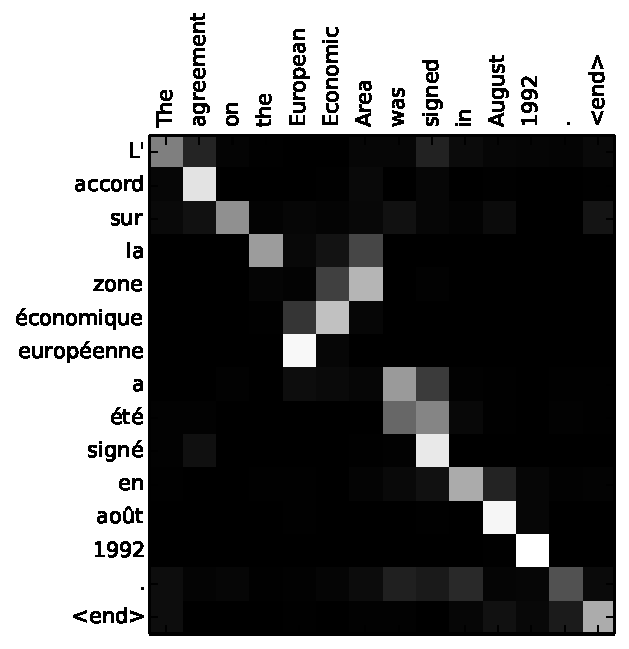
\includegraphics[width=0.6\linewidth]{query_expansion/attention_matrix_example.pdf}
	\caption[Illustration of the attention mechanism via the score matrix of an attention-based neural machine translation model.]{
		%
		An attention matrix $M$ of an attention-based neural machine translation model corresponding to a translation from English (x-axis) to French (y-axis).
		%
		Each cell $M_{ij}$ denotes the importance of the $j$-th word in the source sentence when the model is producing the $i$-th word in the target sentence, with white being the highest score and black being the lowest score.
		%
		We can observe that most of the time the model only looked at a few source words while ignoring the rest, and that the there is a linear alignment between the source and the target texts.
		%
		Interestingly, the entity \emph{European Economic Area} was translated to \emph{zone économique européenne} in French in a reverse direction, evidently shown by the attention matrix.
	}
	\label{fig:attention_illustration}
\end{figure}


\subsection{Attention Mechanism}
\label{sec:related_attention}

%
Early work in neural machine translation~\cite{luong2015effective, bahdanau2014neural} revealed and refined a novel soft alignment technique called \emph{attention}, which becomes a significant contribution in NLP and lays the foundation for many recent advances in natural language processing~\cite{vaswani2017attention, devlin2019bert}, computer vision~\cite{dosovitskiy2020image, liu2021swin} and reinforcement learning~\cite{tang2020neuroevolution, shen2019self}.
%
The attention mechanism is proposed to mimic the excellent human capability of paying attention only to the relevant parts when presented with a piece of information (e.g., an image or a text passage).
%
The idea is to guide the model to focus on those small but important pieces of evidence as it reads in the input sequence.
%
This can be best illustrated using an example in~\fref{fig:attention_illustration}.
%
Each cell $M_{ij}$ in the attention matrix denotes attention scores of a neural machine translation model assigning to the $j$-th word in the source sentence when translating the $i$-th word in the target sentence.
%
It is clear that most of the time, the model only looked at a single word in the source sentence that is one-to-one translated to the words in the target sentence.
%
By employing the attention mechanism, the model is allowed to ignore certain parts of the input sequence that are deemed irrelevant, and instead focus on relevant ones.
%
It is important to highlight that the attention mechanism has become ubiquitous in deep learning recently due to the tremendous performance gain it brings about with little extra computational cost, and has transformed into many variants such as self-attention or cross-attention.
%
We advance these observations one step further and propose a technique that takes advantage of cross-attention scores in an unsupervised manner to extract salient keywords from texts, which will be described later in~\sref{sec:query_expansion_method}.


\subsection{Synthetic Data Generation}


Synthetic data approaches aim at generating a set of artificially synthesized samples from the real, original data while trying to retain as much statistical distribution of the original data as possible.
%
Synthetic data generation has become increasingly predominant in the deep learning research community~\cite{wang2019learning, tripathi2019learning, lacoste2020synbols}, especially in the domains where the data is scarce such as medical treatment~\cite{chen2021synthetic, frid2018synthetic}.
%
Over the past decade, numerous synthetic data generation techniques have been proposed to tackle many aspects of machine learning, from early forms such as data augmentation~\cite{shorten2019survey, tran2017bayesian} or computer simulation~\cite{richter2016playing, song2017semantic} to more recent advances such as Generative Adversarial Networks (GANs)~\cite{goodfellow2014generative, karras2020analyzing} or pseudo data generation~\cite{arazo2020pseudo, wang2020unsupervised}.
%
Existing work in OpenQA adopted synthetic answer generation and question generation to improve the performance of existing state-of-the-art models in two main ways: \emph{unsupervised pre-training} and \emph{query augmentation}.


\subsection{Unsupervised Pre-training}
\label{sec:unsupervised_pre_training}


\begin{figure}[!ht]
	\centering
	
	\subfloat[Masked Language Modeling (Masked LM)]{%
		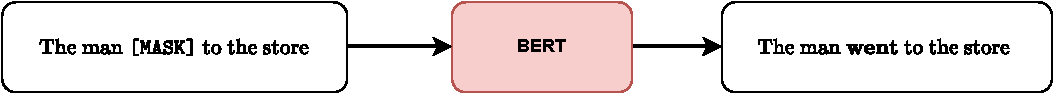
\includegraphics[clip,width=0.8\columnwidth]{query_expansion/masked_lm.pdf}%
	}
	\vspace{0.5cm}
	
	\subfloat[Next Sentence Prediction (NSP)]{%
		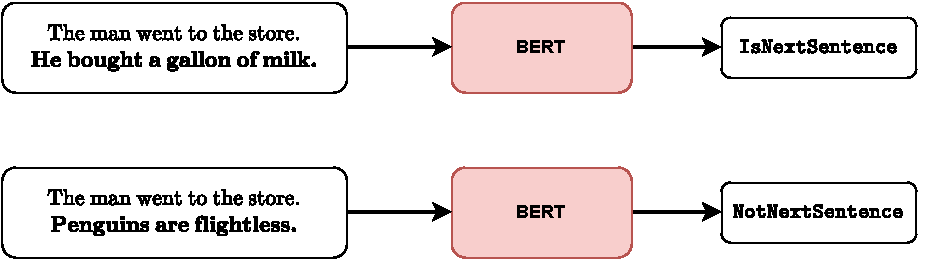
\includegraphics[clip,width=0.7\columnwidth]{query_expansion/next_sentence_prediction.pdf}%
	}
	\caption[BERT~\cite{devlin2019bert} unsupervised training objectives.]{
		%
		BERT~\cite{devlin2019bert} unsupervised training objectives.
		%
		With Masked LM, the model is asked to predict words that have been masked out of the sentence.
		%
		With Next Sentence Prediction, the model is asked to predict if a sentence is the grammatically and semantically possible next sentence of another sentence.
	}
	\label{fig:unsupervised_pretraining_bert}
\end{figure}


%
Together with the attention mechanism, \emph{unsupervised pre-training} has become a must-have recipe in natural language processing that contributes to recent rapid development in the field.
%
It all starts from the paper~\citet{devlin2019bert} which proposed to pre-train deep bidirectional transformer~\cite{vaswani2017attention} models on large unlabeled corpora of texts such as Wikipedia or Common Crawl.
%
In unsupervised pre-training, we are supplied with huge corpora of texts that can be easily crawled from the Internet, from which the models are required to perform natural language reasoning and understanding without any supervision.
%
This is made possible by carefully designed unsupervised objective functions, namely \emph{Masked Language Model} (Masked LM) and \emph{Next Sentence Prediction} (NSP).
%
\fref{fig:unsupervised_pretraining_bert} present illustrative examples of input-output pairs of the unsupervised training paradigm.
%
In Masked LM, a portion of the input text sequence is masked out using a special token $\texttt{[MASK]}$, for which the model is trained to predict the correct corresponding unmasked words.
%
On the other hand, Next Sentence Prediction takes a pair of consecutive sentences and randomly replaces the second sentence with another random sentence from the corpus.
%
The model is then trained to classify whether the latter sentence reasonably comes after the former sentence.
%
Importantly, unsupervised pre-training play a crucial role in many recent successes in deep learning~\cite{devlin2019bert, brown2020language, caron2020unsupervised, goyal2021self}, especially in the era of big data where unlabeled data can be obtained with virtually no effort.


\paragraph{Synthetic data training/pre-training}
%
In OpenQA, pre-training models with synthetic corpora has attracted increasing attention from researchers recently because it allows to observe much larger, more diverse datasets to improve model generalizability and performance.
%
\citet{alberti2019synthetic} used a sequence-to-sequence~\cite{sutskever2014sequence} model to generate synthetic questions from passages and a reading comprehension model to verify question answerability.
%
\citet{lewis2019unsupervised} sampled random nouns or entities from passages to generate a synthetic dataset of fill-in-the-blank cloze questions, which are then translated to natural questions using an unsupervised neural machine translation model.
%
This work showed that models trained on only synthetic data are able to achieve decent performance, testifying to the usability of generated data.
%
\citet{lewis2021paq} introduced a huge dataset of 65 million synthetic question-answer pairs using a sophisticated data generation pipeline.
%
A simple QA-pair retriever model trained on this dataset is able to match the performance of a two-stage retriever-reader model while being significantly faster.
%


\subsection{Query Augmentation}
%
In OpenQA, query augmentation techiques aim at preempting the query questions with relevant information, thus are expected to improve the retrieval stage substantially.
%
This technique is especially useful for multi-hop retrieval which requires information aggregation and complex reasoning over multiple pieces of evidence.
%
Given an input question, instead of trying to retrieve seemingly-unrelated related documents, we can enrich the query with relevant keywords retrieved from a pre-cached parametric memory.
%
It is important to note that to possibly incorporate all question-keywords pairs of a knowledge base to such memory, one must train a sequence-to-sequence model on a generated synthetic dataset that sufficiently covers all relationships within the knowledge base.
%
\citet{qi2019answering} proposed to iteratively enrich the query with progressively obtained keywords from previous steps to tackle the task of multi-hop open-domain question answering.
%
\citet{mao2021generation} demonstrated the advantages of query augmentation by performing only sparse retrieval using augmentated queries, achieving comparable performance as more computationally costly dense retrieval methods.

%
In this work, we take advantage of a huge synthetic question answering dataset for both synthetic data pre-training and query augmentation, which we will describe in detail in \sref{sec:query_expansion_method}.



\section{Method}
\label{sec:query_expansion_method}


\begin{figure}[!htbp]
	\centering
	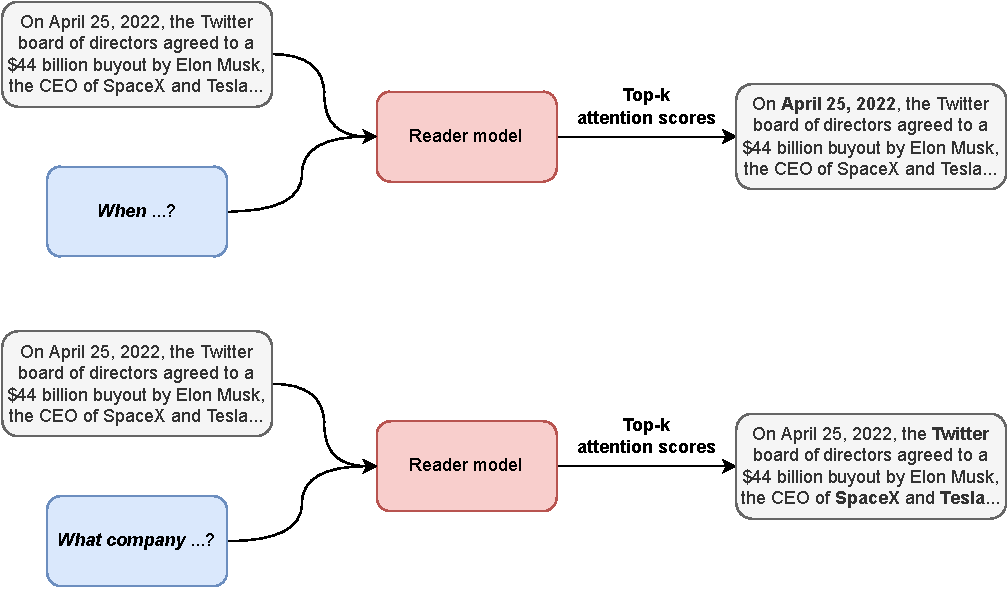
\includegraphics[width=0.95\linewidth]{query_expansion/question_type_specific.pdf}
	\caption[Illustration of the idea of unsupervised keyword extraction.]{
		%
		Illustration of the idea of unsupervised keyword extraction using a trained reader model.
		%
	 	When presented with a \emph{when} question, the model pays most attention to timestamps in the input passage (e.g., \emph{Apr 25, 2022}).
	 	%
	 	On the other hand, the model answer to a \emph{what company} question by attending to company names in the same input passage (e.g., \emph{Twitter}, \emph{SpaceX}, and \emph{Tesla}).
	}
	\label{fig:unsupervised_keyword_extraction}
\end{figure}


\subsection{Unsupervised Keyword Extraction}
\label{sec:unsupervised_keyword_extraction}
%
In this step, we generate salient keywords from passages in an unsupervised manner by exploiting attention scores as described in~\sref{sec:related_attention}.
%
This process is motivated by the observation that when generating an answer to a question, the generative reader model must pay attention to question type-specific tokens in the given relevant context passages.
%
\fref{fig:unsupervised_keyword_extraction} illustrates this idea, from which we observe that the model considers different sets of keywords highly depedent on the input question type.

%
In particular, suppose we have a large corpus $\mathcal{C}$ of $K$ factual documents $\{p_1, p_2, \ldots, p_K\}$, e.g., Wikipedia.
%
Furthermore, we are given a trained generative reader $M$ which is a encoder-decoder transformer-based~\cite{vaswani2017attention} model.
%
When we supply the model with a wh-question word $w$ (e.g., \emph{who}) and a context passage $p \in \mathcal{C}$ consisting of $n$ tokens $\{p^{(1)}, p^{(2)}, \ldots, p^{(n)}\}$, concatenated into a single sequence (e.g., \emph{$\text{who} \texttt{ [SEP] } p^{(1)} \text{ } p^{(2)} \text{ } \ldots \text{ } p^{(n)}$}), we can obtain the attention-based score matrices as intermediate products of the cross-attention mechanism \emph{when the model is generating the first token in the decoder side} as
%
\begin{equation}
%
\mathbf{Q} \in \mathbb{R}^{1 \times d}, \mathbf{K} \in \mathbb{R}^{n \times d}, \mathbf{V} \in \mathbb{R}^{n \times d}
\end{equation}
%
where $d$ is the feature dimension.
%
Here we have $\mathbf{Q}$ as the query matrix in the decoder side, as well as $\mathbf{K}$ and $\mathbf{V}$ as the key and value matrices, respectively, in the encoder side.
%
The cross-attention scores between the first token in the ouput sequence and each of the tokens in the input sequence are computed as
%
\begin{equation}
\text{Attention}(\mathbf{Q}, \mathbf{K}, \mathbf{V}) = \text{softmax}(\mathbf{Q} \cdot \mathbf{K}^{T}) \cdot \mathbf{V} \in \mathbb{R}^{1 \times d}
\end{equation}
%
where $\text{softmax}$ is the softmax activation function defined in~\eqref{def:softmax}~\footnote{We omit the scaling factor for brevity}.
%
We refer interested readers to~\citet{vaswani2017attention} for a complete description and discussion of attention mechanisms.
%
Notice that we can omit the value matrix $\mathbf{V}$ and instead define
\begin{equation}
\text{Relevance}(\mathbf{Q}, \mathbf{K}) = \text{softmax}(\mathbf{Q} \cdot \mathbf{K}^{T}) \in \mathbb{R}^{1 \times n}
\end{equation}
%
as the \emph{relevance score vector}, where the $i$-th value in the vector denotes how relevant the $i$-th input token $p^{(i)}$ is when generating the first token in the answer, which is utimately based on the given question type $w$.
%
In practice, the transformer-based model~\cite{vaswani2017attention} often comprises of multiple attention heads (so-called multi-head attention).
%
This means that we can obtain $M$ sets of query-keyword matrices $\{(\mathbf{Q}_1, \mathbf{K}_1), (\mathbf{Q}_2, \mathbf{K}_2), \ldots, (\mathbf{Q}_M, \mathbf{K}_M)\}$.
%
We take advantage of the complementary power of these heads and compute the relevance scores by simply marginalizing over all heads as
%
\begin{equation}
\text{Relevance}(\mathbf{Q}, \mathbf{K}) = \frac{1}{M} \sum_{i=1}^{M} \text{softmax}(\mathbf{Q}_i \cdot \mathbf{K}^{T}_i) \in \mathbb{R}^{1 \times n}
\end{equation}
%
We then simply take tokens with the highest attention-based relevance scores based on the computed relevance vector as our \emph{extracted keywords}
%
\begin{equation}
\text{keyword\_extraction}(w, p^{(1)}, p^{(2)}, \ldots, p^{(n)}) = \text{top\_k}(\text{Relevance}(\mathbf{Q}, \mathbf{K}))
\end{equation}

\begin{figure}[!htbp]
	\centering
	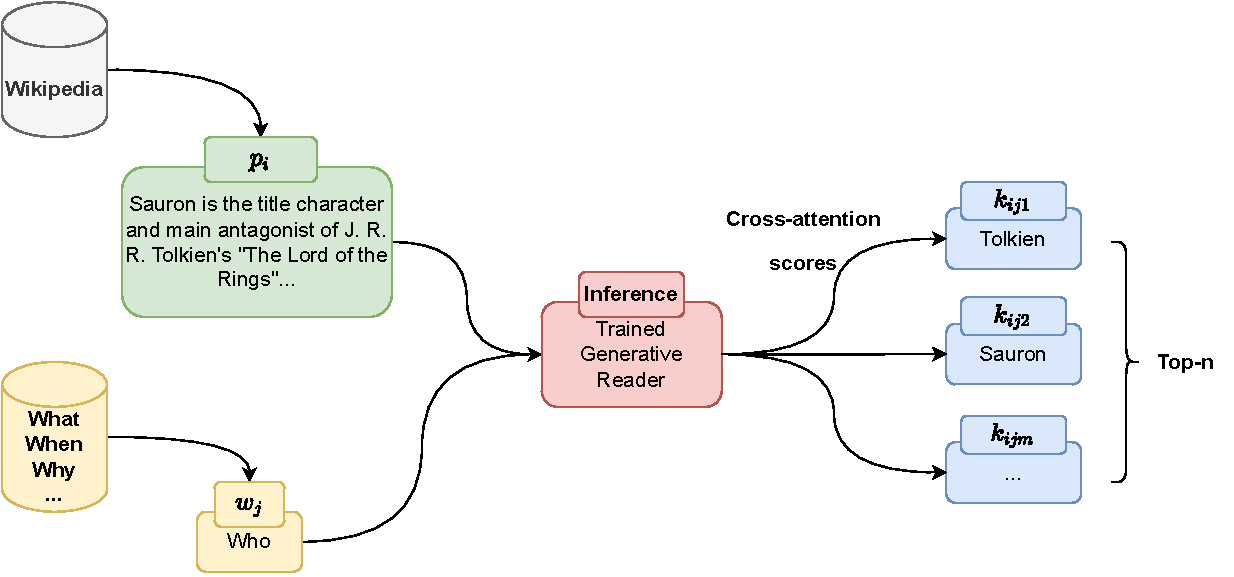
\includegraphics[width=0.95\linewidth]{query_expansion/unsupervised_keyword_extraction.pdf}
	\caption[Illustration of the unsupervised keyword extraction pipeline.]{
		%
		Illustration of the unsupervised keyword extraction pipeline.
		%
		For each passage $p_i$ in the Wikipedia corpus and each question type $w_j$, we generate a set of question-type-specific keywords $\{k_{ij1}, k_{ij2}, \ldots, k_{ijm}\}$ based on the cross-attention scores.
	}
	\label{fig:unsupervised_keyword_extraction_pipeline}
\end{figure}

%
In practice, we first analyze the Natural Questions dataset to obtain a set of commonly asked question types $\{w_1, w_2, \ldots\}$.
%
We then perform this unsupervised keyword extraction step on the entire Wikipedia corpus, obtaining a set of $m$ keywords $\{k_{ij1}, k_{ij2}, \ldots, k_{ijm}\}$ for each combination of passage $p_i$ and question type $w_j$, as illustrated in~\fref{fig:unsupervised_keyword_extraction_pipeline}.


\begin{figure}[!htbp]
	\centering
	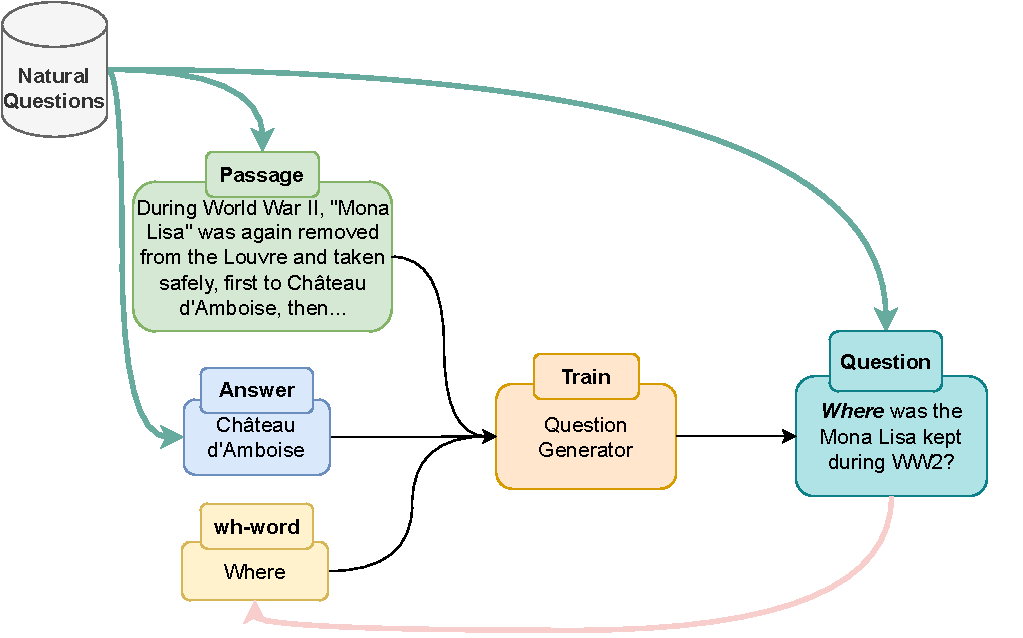
\includegraphics[width=0.8\linewidth]{query_expansion/question_generator_train.pdf}
	\caption[Illustration of the question generator training pipeline.]{
		%
		Illustration of the question generator training pipeline.
		%
		The model is trained to generate a plausible question given a context passage, an answer and a question type.
		%
		Different from existing work, we infer the question type from the questions use it as one of the supervised signals.
	}
	\label{fig:question_generator_train}
\end{figure}


\subsection{Question Generation}
\label{sec:question_generation_method}
%
Following existing work on synthetic question generation~\cite{alberti2019synthetic, chan2019recurrent, sultan2020importance, lewis2021paq}, we train a question generator model using supervised information from the Natural Questions dataset as shown in~\fref{fig:question_generator_train}.
%
However, we also provide the model with the question types of the target questions, thereby enhancing the capability of the model at generating plausible questions with an additionaly input signal, as well as more diverse questions with various question prompts.
%

\begin{figure}[!htbp]
	\centering
	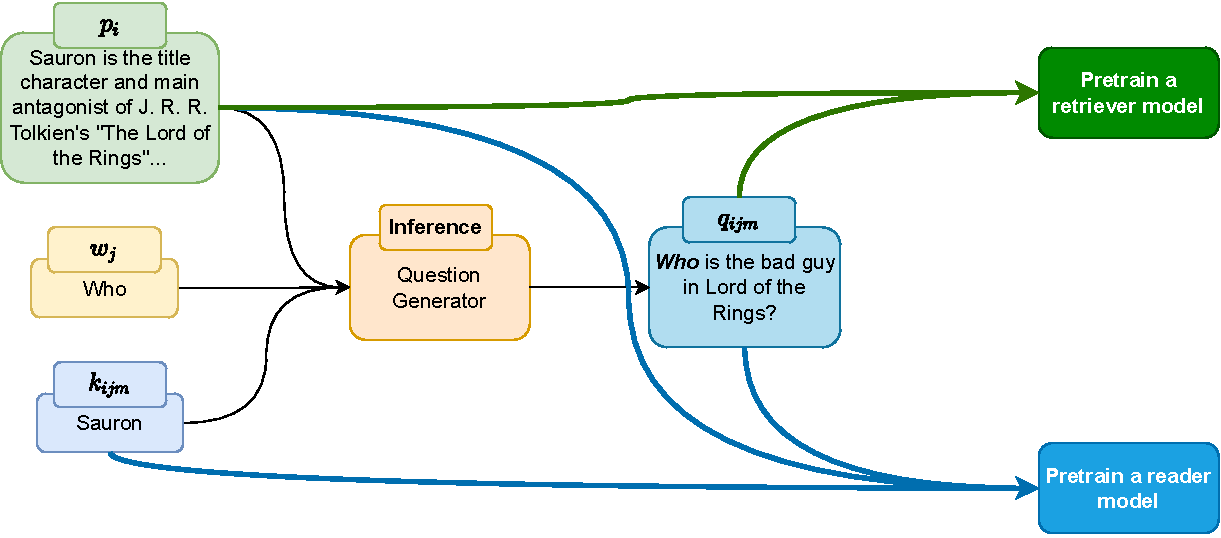
\includegraphics[width=\linewidth]{query_expansion/question_generator_inference.pdf}
	\caption[Illustration of the question generator inference pipeline.]{
		%
		Illustration of the question generator inference pipeline.
		%
		We take the trained question generator model to synthesize questions for passage-question type-keyword pairs obtained from the unsupervised keyword extraction step~\sref{sec:unsupervised_keyword_extraction}.
	}
	\label{fig:question_generator_inference}
\end{figure}

%
After finished, the trained question generator model will be used to infer a synthetic question $q_{ijm}$ for each combination of passage $p_i$, question type $w_j$ and keyword $k_{ijm}$ obtained from the unsupervised keyword extraction step~\sref{sec:unsupervised_keyword_extraction}.
%
This is illustrated in~\fref{fig:question_generator_inference}.
%
By doing so, we obtain an enormous, high-quality synthetic dataset of (passage $p_i$, question $q_{ijm}$, answer $k_{ijm}$) pairs.
%
This synthetic dataset can be used to pre-train both the retriever and reader model in the two-stage retriever-reader framework described in~\sref{sec:open_book}, following the procedure and conventions described in~\sref{sec:unsupervised_pre_training} in an unsupervised manner.

\subsection{Query Expansion}
\label{sec:query_expansion_submethod}



\begin{figure}[!ht]
	\centering
	
	\subfloat[Training]{%
		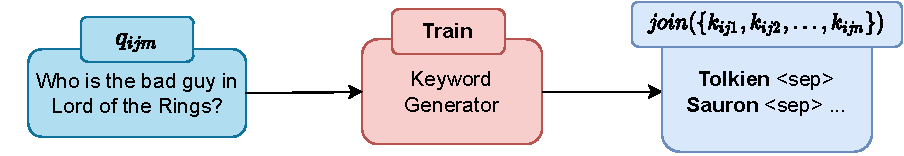
\includegraphics[clip,width=0.7\columnwidth]{query_expansion/query_expansion_method.pdf}%
	}
	\vspace{0.5cm}
	
	\subfloat[Inference]{%
		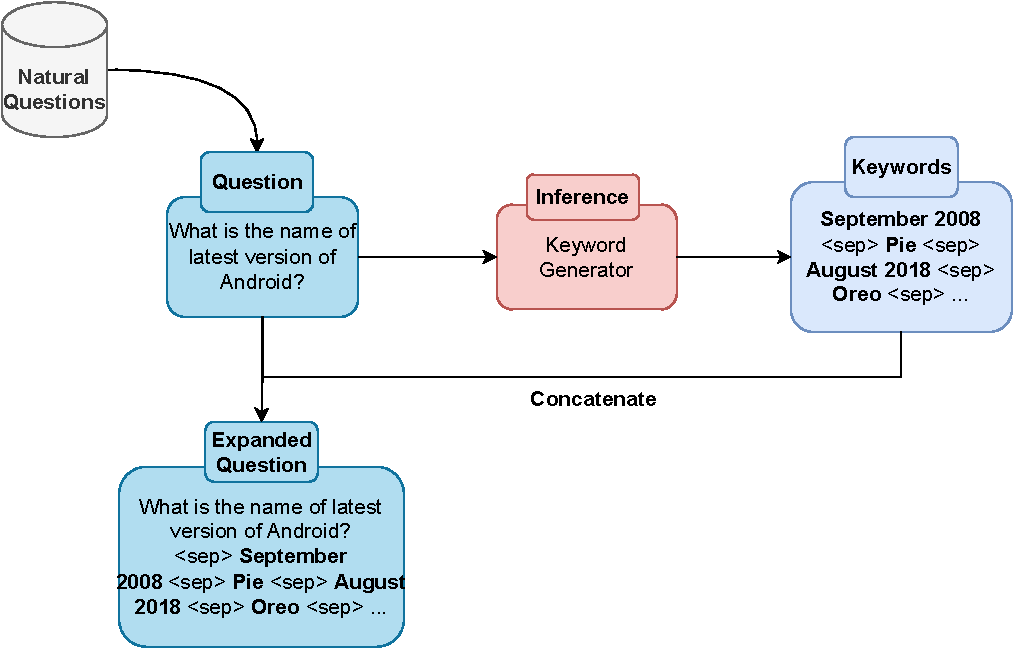
\includegraphics[clip,width=0.8\columnwidth]{query_expansion/query_expansion_method_inference.pdf}%
	}
	\caption[Illustration of the query expansion training and inference pipelines.]{
		%
		Illustration of the query expansion training and inference pipelines.
	}
	\label{fig:query_expansion_pipeline}
\end{figure}


The query expansion training and inference pipelines are illustrated in~\fref{fig:query_expansion_pipeline}.


\section{Experimental Results}
\label{sec:query_expansion_results}


We managed to implement and experiment with the processes of \emph{unsupervised keyword extraction} (\sref{sec:unsupervised_keyword_extraction}), \emph{question generation} (\sref{sec:question_generation_method}) as well as unsupervised retriever and reader pre-training (\sref{sec:question_generation_method}).

\begin{table*}[t!]
	\setlength\tabcolsep{5pt}
	\centering
	\small
	\begin{tabular}{ll|cc}
		\toprule
		\textbf{Architecture} & \textbf{Model}
		& Top-20 & Top-100 \\ 
		\midrule
		\multirow{3}{*}{\shortstack{DPR retriever~\cite{karpukhin2020dense}}} 
		& Original (real) & 78.4 & 85.4  \\
		& Pre-trained (synthetic) & 70.2 & 81.5 \\
		& Pre-trained (synthetic) + fine-tune (real) & \textbf{80.5} & \textbf{86.7} \\
		\bottomrule
	\end{tabular}
	\caption[Top-$\{20, 100\}$ retrieval accuracy on the Natural Questions test set of the DPR retriever with and without unsupervised pre-training.]{
		%
		Top-$\{20, 100\}$ retrieval accuracy on the Natural Questions test set of the DPR retriever with and without unsupervised pre-training
	}
	
	\label{tab:retriever_unsupervised_pretraining}
\end{table*}



\begin{table*}[t!]
	\setlength\tabcolsep{5pt}
	\centering
	\small
	\begin{tabular}{ll|c}
		\toprule
		\textbf{Architecture} & \textbf{Model}
		& Exact Match \\ 
		\midrule
		\multirow{3}{*}{\shortstack{DPR reader~\cite{karpukhin2020dense}}} 
		& Original (real) & 41.5  \\
		& Pre-trained (synthetic) & 28.4 \\
		& Pre-trained (synthetic) + fine-tune (real) & \textbf{44.4} \\
		\bottomrule
	\end{tabular}
	\caption[Top-$\{20, 100\}$ retrieval accuracy on the Natural Questions test set of the DPR reader with and without unsupervised pre-training.]{
		%
		Top-$\{20, 100\}$ retrieval accuracy on the Natural Questions test set of the DPR reader with and without unsupervised pre-training
	}
	
	\label{tab:reader_unsupervised_pretraining}
\end{table*}




\begin{table*}[t!]
	\setlength\tabcolsep{5pt}
	\centering
	\small
	\begin{tabular}{ll|c}
		\toprule
		\textbf{Architecture} & \textbf{Model}
		& Exact Match \\ 
		\midrule
		\multirow{3}{*}{\shortstack{FiD reader~\cite{izacard2021leveraging}}} 
		& Original (real) & 48.2  \\
		& Pre-trained (synthetic) & 32.8 \\
		& Pre-trained (synthetic) + fine-tune (real) & \textbf{49.8} \\
		\bottomrule
	\end{tabular}
	\caption[Top-$\{20, 100\}$ retrieval accuracy on the Natural Questions test set of the FiD reader~\cite{izacard2021leveraging} with and without unsupervised pre-training.]{
		%
		Top-$\{20, 100\}$ retrieval accuracy on the Natural Questions test set of the FiD reader with and without unsupervised pre-training
	}
	
	\label{tab:fid_reader_unsupervised_pretraining}
\end{table*}


The results are presented in~\tref{tab:retriever_unsupervised_pretraining},~\tref{tab:reader_unsupervised_pretraining} as well as~\tref{tab:fid_reader_unsupervised_pretraining}.
%!TEX root=../mythesis.tex
% Chapter Template

\chapter{Conclusion} % Main chapter title
\chaptermark{Conclusion}  % replace the chapter name with its abbreviated form
\label{ch:conclusion}


%
Open-domain question answering (OpenQA), the task of answering information-seeking question about nearly anything given a large knowledge base, has attracted tremendous attention from both the research community and the industry due to its impactful applications yet under-explored challenging problems.
%
In this final year project, our goal is to further advance the progress of current OpenQA systems by developing various mathematical-driven approaches.
%
More specifically, we take the landmark work of Dense Passage Retrieval~\cite{karpukhin2020dense} (DPR) as the baseline, on which we perform a comprehensive error analysis to identify model weaknesses.
%
We then propose several novel techniques that are designed to solve one model weakness at a time.

%
First, we introduce the simple parameter sharing idea on top of the DPR retriever in~\cref{ch:shared_encoders}, which is evidently shown to be consistently and substantially more efficient and effective than the baseline.
%
We then aim to tackle the long-standing \emph{decomposability gap} problem of two-stage OpenQA systems by proposing a late interaction module in~\cref{ch:late_interaction}, which we show marginally degrade the model performance.
%
Next, we take the idea of in-batch negatives~\cite{karpukhin2020dense} one step further and propose a novel objective function termed \emph{multi-similarity loss} in~\cref{ch:multi_similarity}.
%
This loss function efficiently takes into account all question-passage, question-question and passage-passage similarities without incurring additional computational overhead, thereby improving over the baseline model by a small margin.
%
Finally, in~\cref{ch:harder_inbatch_negatives} we introduce a novel batch construction technique named \emph{harder in-batch negatives} that groups similar samples into the same batch.
%
By providing a much stronger, more informative signal for retrieval training, our proposed approach is able to speed up the convergence, achieving significant improvements over the DPR retriever.


%----------------------------------------------------------------------------------------
%	THESIS CONTENT - APPENDICES
%----------------------------------------------------------------------------------------

\addtocontents{toc}{\vspace{0.8em}} % Add a gap in the Contents, for aesthetics

\appendix % Cue to tell LaTeX that the following 'chapters' are Appendices

% Include the appendices of the thesis as separate files from the Appendices folder
% Uncomment the lines as you write the Appendices

%!TEX root=../mythesis.tex
% Appendix A

%\chapter{Proofs for Part I or Chapter 3} % Main appendix title
%
%\label{AppendixA} % For referencing this appendix elsewhere, use \ref{AppendixA}
%
%%\lhead{Appendix A. \emph{Appendix Title Here}} % This is for the header on each page - perhaps a shortened title
%\section{Proof of Lemma}
%\label{pf:ApprGradSys}
%
%$$\psi^{av}(\theta)=\frac{1}{T}\int^{T}_0[\psi(\theta+\mu(\tau))+C]\otimes\frac{\mu(\tau)}{a}d\tau$$ 
%
%
%
%\section{Proof of another Lemma}
%\begin{equation}
%\begin{aligned}
%\gamma_1(\left\|x\right\|)\leq W(t,x)\leq \gamma_2(\left\|x\right\|)\\
%\frac{\partial{W}}{\partial{t}}+\frac{\partial{W}}{\partial{x}}\phi(t,x,0)\leq-\gamma_3(\left\|x\right\|)
%\end{aligned}
%\end{equation}

%\input{./Appendices/AppendixB}

% \cleardoublepage    % start a new page

%----------------------------------------------------------------------------------------
%	AUTHOR'S PUBLICATIONS
%----------------------------------------------------------------------------------------

%\authorpublications{
%
%\section*{Awards}
%
%\begin{itemize}
%	\item \textbf{Best Paper Awards}, ``A Great System,'' \emph{Nature}.
%\end{itemize}
%
%\section*{Patents}
%\begin{itemize}
%	\item \textbf{A Great System}, ``A Great System,'' \emph{Nature}.
%\end{itemize}
%
%\section*{Journal Articles}
%
%\begin{itemize}
%    \item \textbf{My name} and My colleague, ``A Great System,'' \emph{Nature}.
%\end{itemize}
%
%\section*{Conference Proceedings}
%
%\begin{itemize}
%  \item \textbf{My name}, My colleague 1, My colleague 3 and My colleague 3, ``Greater System,'' in \emph{Conference of Vision, 2018}.
%\end{itemize}
%
%}
%
%\backmatter

%----------------------------------------------------------------------------------------
%	BIBLIOGRAPHY
%----------------------------------------------------------------------------------------

\label{Bibliography}
\setstretch{1}
\bibliographystyle{unsrtnat}
\bibliography{references.bib}

\end{document}
